\documentclass[12pt,a4paper,bibliography=totocnumbered,listof=totocnumbered]{scrartcl}
\usepackage[ngerman]{babel}
\usepackage[utf8]{inputenc}
\usepackage[numbers,square]{natbib}
\usepackage{amsmath}
\usepackage{amsfonts}
\usepackage{amssymb}
\usepackage{graphicx}
\usepackage[export]{adjustbox}
\usepackage{fancyhdr}
\usepackage{tabularx}
\usepackage{geometry}
\usepackage{setspace}
\usepackage[right]{eurosym}
\usepackage{acronym}
\usepackage{subfigure}
\usepackage{floatflt}
\usepackage[usenames,dvipsnames]{color}
\usepackage{colortbl}
\usepackage{paralist}
\usepackage{array}
\usepackage[right]{eurosym}
\usepackage[subfigure,titles]{tocloft}
\usepackage[pdfpagelabels=true]{hyperref}
\usepackage{listings}
\usepackage{eurosym}
\usepackage{textcomp}
\usepackage{pdfpages} 
\usepackage{tabularx}
\usepackage{ragged2e}
\usepackage{xcolor}
\usepackage{hyperref}

\geometry{a4paper, top=27mm, left=30mm, right=20mm, bottom=35mm, headsep=10mm, footskip=12mm}

\hypersetup{unicode=false, pdftoolbar=true, pdfmenubar=true, pdffitwindow=false, pdfstartview={FitH},
	colorlinks=true,linkcolor=black,citecolor=black,filecolor=magenta,urlcolor=black}

\begin{document}

% Kopf- und Fusszeile
\renewcommand{\sectionmark}[1]{\markright{#1}}
\renewcommand{\leftmark}{\rightmark}
\pagestyle{fancy}
\lhead{}
\chead{}
\rhead{\thesection\space\contentsname}
\lfoot{Abschlussbericht\newline Automatische Werkzeug-Kontakt Detektion}
\cfoot{}
\rfoot{\ \linebreak Seite \thepage}
\renewcommand{\headrulewidth}{0.4pt}
\renewcommand{\footrulewidth}{0.4pt}

% Vorspann 
\pagenumbering{Roman}

% ----------------------------------------------------------------------------------------------------------
% Titelseite
% ----------------------------------------------------------------------------------------------------------
\thispagestyle{empty}
\begin{center}
	\vspace*{2cm}
	\Large
	\textbf{Fachbereich 4}\\
	\textbf{Produktionstechnik -Maschinenbau \& Verfahrenstechnik}\\
	\vspace*{2cm}
	\Huge
	\textbf{Abschlussbericht des Systemtechnikprojektes im Studiengang Systems Engineering}\\
	\vspace*{0.5cm}
	\Large
	Automatische Werkzeug-Kontakt Detektion\\
	
	\vfill
	\normalsize
	\newcolumntype{x}[1]{>{\raggedleft\arraybackslash\hspace{0pt}}p{#1}}
	\begin{tabular}{x{6cm}p{7.5cm}}
		\rule{0mm}{5ex}\textbf{Autoren:} & Kira Löper\\ 
		& Erik Rother\\
		& Lisa Schade
		\\
		\rule{0mm}{5ex}\textbf{Lehrender:} & Prof. Dr. Ekkard Brinksmeier \\ 
		\rule{0mm}{5ex}\textbf{Tutoren:} & M. Sc Timo Dörgeloh\\&M. Sc Ann-Katrin Holthusen \\ 
		\rule{0mm}{5ex}\textbf{Abgabedatum:} & \today \\ 
	\end{tabular} 
\end{center}
\pagebreak
%eidesstattliche
\newpage
\section*{Erklärung}
\thispagestyle{empty}
\vspace{2em}
\justifying
Hiermit versichere ich, dass ich die vorliegende schriftliche Hausarbeit selbständig angefertigt habe. Alle Stellen, die dem Wortlaut oder dem Sinn nach anderen Werken (einschließlich elektronischer Quellen) entnommen sind, habe ich in jedem einzelnen Fall unter genauer Angabe der Quelle deutlich gekennzeichnet.\\

\vspace{1cm}
\begin{minipage}{\linewidth}
	\begin{tabular}{p{15em}p{15em}}
		Datum: .........................&  .......................................................\\
		& Kira Löper
	\end{tabular}
\end{minipage}\vspace{0.5cm}

\vspace{1cm}
\begin{minipage}{\linewidth}
	\begin{tabular}{p{15em}p{15em}}
		Datum: .........................&  .......................................................\\
		& Erik Rother
	\end{tabular}
\end{minipage}\vspace{0.5cm}

\vspace{1cm}
\begin{minipage}{\linewidth}
	\begin{tabular}{p{15em}p{15em}}
		Datum: .........................&  .......................................................\\
		& Lisa Schade
	\end{tabular}
\end{minipage}\vspace{0.5cm}
\newpage
% ----------------------------------------------------------------------------------------------------------
% Verzeichnisse
% ----------------------------------------------------------------------------------------------------------
% TODO Typ vor Nummer
\renewcommand{\cfttabpresnum}{Tab. }
\renewcommand{\cftfigpresnum}{Abb. }
\settowidth{\cfttabnumwidth}{Abb. 10\quad}
\settowidth{\cftfignumwidth}{Abb. 10\quad}

\singlespacing
\rhead{INHALTSVERZEICHNIS}
\tableofcontents
\pagebreak
% ----------------------------------------------------------------------------------------------------------
% Inhalt
% ----------------------------------------------------------------------------------------------------------


% Kopfzeile
\renewcommand{\sectionmark}[1]{\markright{#1}}
\renewcommand{\subsectionmark}[1]{}
\renewcommand{\subsubsectionmark}[1]{}
\lhead{Kapitel \thesection}
\rhead{\rightmark}

\onehalfspacing
\renewcommand{\thesection}{\arabic{section}}
\renewcommand{\theHsection}{\arabic{section}}
\setcounter{section}{0}
\pagenumbering{arabic}
\setcounter{page}{1}

\section{Einleitung}
In der Mikrostrukturierung optischer Bauteile werden Diamantwerkzeuge mit sehr kleinen Schneidenradien eingesetzt. Die Detektion des Werkzeugkontaktes kann nur durch eine Kamera realisiert werden. Die genau Positionierung der Kamera und die Veränderung der Position sind sehr zeitaufwändig. Während unseres Projektes haben wir uns mit diesem Problem beschäftigt und als Lösung eine elektrisch gesteuerte Kameraführung mit automatischer Werkzeugdetektion entwickelt. In diesem Bericht möchten wir den Prozess der Entwicklung und unsere Resultate beschreiben. 

\section{Stand der Technik}
Die automatische Werkzeug-Kontakt-Detektion dient zur Unterstützung der Werkzeug-Positionierung bei mehreren Prozessen. Im Folgenden werden zwei Prozesse vorgestellt, die durch die automatische Werkzeug-Kontakt-Detektion zeiteffizienter gestaltet werden können. \\ \\
Zur Einordnung dieser Prozesse dient Abbildung 1. Es sind einige Verfahren zur Herstellung strukturierter optischer Komponenten nach ihrer Komplexität sortiert aufgeführt. Des Weiteren kann man der Abbildung ihre Dimensionen und Anwendungen entnehmen. \\ \\ 
\begin{figure}[htbp]
\centering 
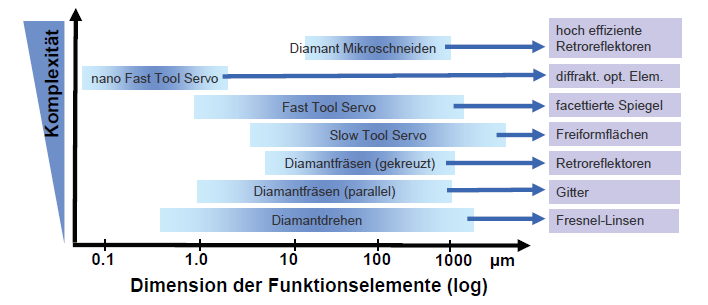
\includegraphics[width=0.8\textwidth]{Fertigungsverfahren.PNG}
\caption[Gla09]{Werkzeug zum Mikroschneiden}
\label{fig:Bild1}
\end{figure}
\break

\subsection{Diamant-Mikroschneiden}
Das Diamant-Mikroschneiden dient zur Herstellung von prismatischen Mikrokavitäten mit scharfkantig aufeinandertreffenden Facettenflächen, wie sie zum Beispiel bei retroreflektierenden Strukturen erforderlich sind. Um retroreflektierende Strukturen zu fertigen werden aus glatten Oberflächen gezielt bestimmte Bereiche entfernt und die reflektierende Struktur bleibt stehen. Das Diamant-Mikroschneiden unterschiedet sich durch seine Werkzeuge und Kinematik grundlegend von anderen Fertigungsverfahren. \\ \\
Abbildung 2 zeigt das Diamant-Werkzeug, welches sich dadurch auszeichnet, dass Span-und Freifläche gegeneinander vertauscht wurden. \\ \\
\begin{figure}[htbp]
\centering 
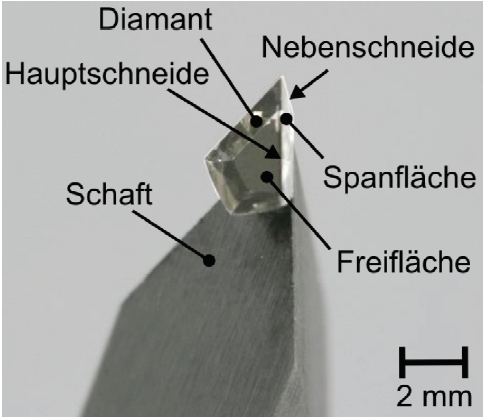
\includegraphics[width=0.3\textwidth]{Werkzeug.PNG}
\caption [Gla09]{Werkzeug zum Mikroschneiden}
\label{fig:Bild2}
\end{figure}
\pagebreak
\\ \\
Abbildung 3 zeigt die Kinematik des Mikroschneidens. Das Werkzeug schneidet zunächst in X,Y,-Z Richtung in das Werkstück und wird anschließend in \\-X,Y,Z Richtung zurückgeführt. Nachfolgend wird das Werkstück rotiert und der Schnittvorgang wiederholt sich. Durch diesen Vorgang können drei- bis sieben-seitige Kavitäten erstellt werden. \\ \\
Außerdem ist die Herstellung von kubischen Retroreflektoren aus dreieckigen Einzelstrukturen abgebildet. \\ \\
\begin{figure}[htbp]
\centering 
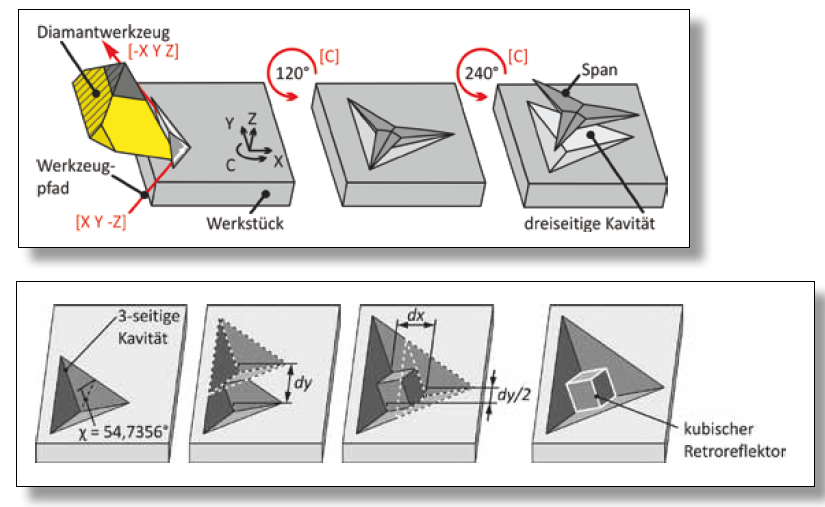
\includegraphics[width=0.7\textwidth]{Mikroschneiden_Kinematik.PNG}
\caption[Sch14]{Kinematik des Mikroschneidens}
\label{fig:Bild3}
\end{figure}
\break
Besonders wichtig beim Mikroschneiden ist die richtige Justierung des Werkzeuges innerhalb der Maschine. Hier muss eine Genauigkeit von unter einem Mikrometer in allen Raumrichtungen erreicht werden. Sonst würden sich die einzelnen Spiegelflächen der Strukturen nicht präzise treffen und die gewünschte optische Funktion ließe sich nicht erreichen.




\subsection{Nano Fast Tool Servos (nFTS)}
Das Verfahren nano Fast Tool Servos dient zur Herstellung diffraktiver optischer Komponenten, welche ihre Anwendung beispielsweise in der Sicherheitstechnik finden. Dieses Verfahren arbeitet mit einer speziellen piezoelektrischen Keramik, welche sich durch eine hohe Linearität und geringe Hysterese auszeichnet. Darauf befindet sich eine Montageplatte für das Diamantwerkzeug. \\ \\
Die herzustellende Strukturgeometrie unterliegt sowohl den Anforderungen des optischen Designs als auch denen der Bearbeitungstechnologie. Um beide möglichst gut zu berücksichtigen wird eine so genannte Blaze-Struktur verwendet. In der folgenden Abbildung 2.4 ist links die Geometrie einer Blaze-Optik zu sehen. Rechts ist eine diffraktive Umsetzung zur Fertigung mit Diamantwerkzeugen abgebildet. Strukturdaten werden als Höhenmodulation in die Flanken eingeschrieben. 
\begin{figure}[htbp]
\centering 
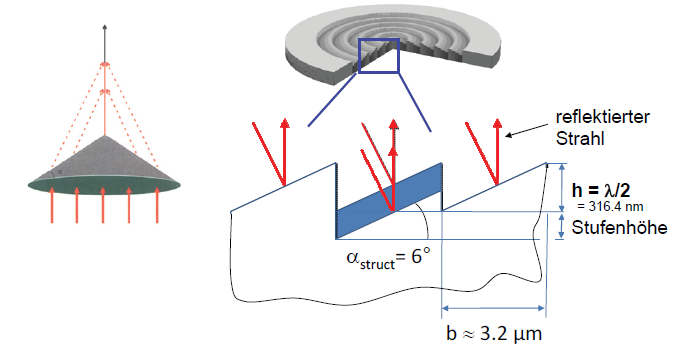
\includegraphics[width=0.7\textwidth]{Blaze_Optik.PNG}
\caption [Gla09]{Blaze-Struktur}
\label{fig:Bild4}
\end{figure}
\break
Nachfolgend ist der Bearbeitungsprozess des nFTS zu sehen. Rechts ist das Diamantwerkzeug, welches bei diesem Verfahren verwendet wird, abgebildet. \\ \\ 
\begin{figure}[htbp]
\centering 
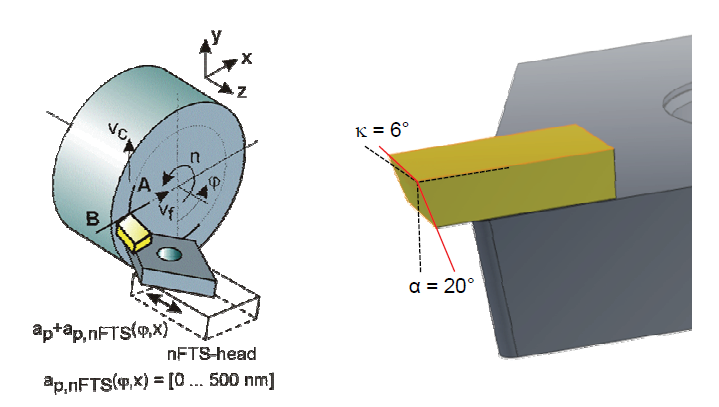
\includegraphics[width=0.6\textwidth]{nano.PNG}
\caption [Gla09]{Bearbeitungsprozess}
\label{fig:Bild5}
\end{figure}
\break
\pagebreak
\\ \\
Beide Prozesse haben hohe Anforderungen an eine genaue Positionierung des Werkzeugs. Außerdem ist das Werkzeug in beiden Fällen aus Diamant, einem sehr teuren Werkstoff. Somit ist es besonders wichtig den Kontakt zwischen Werkzeug und Werkstück vorsichtig herzustellen, sodass es nicht zu Beschädigungen kommt. Dazu ist ein Kamerasystem mit starker Vergrößerung notwendig. Bisher wurde dies mit einer Kamera an der Werkzeughalterung realisiert. Diese musste manuell positioniert werden, wodurch viel Zeit in Anspruch genommen wurde. Während des Bearbeitungsprozesses kann es bei bestimmten Winkeln des Werkzeuges vorkommen, dass das Werkstück nicht mehr im Bildausschnitt zu sehen ist. Dies erfordert eine erneute manuelle Positionierung der Kamera und nimmt wieder Zeit in Anspruch. \\ \\

\section{Konzeptentwicklung}

Nachdem wir uns mit der Problematik der Kamerapositionierung zur Werkzeug-Kontakt-Detektion beschäftigt haben, wurden erste Lösungsansätze erarbeitet. Die grundlegende Fragestellung befasste sich damit, welche Art der Kameraführung am besten für das gegebene Problem geeignet ist. Bei der Beurteilung galt es zu überprüfen, ob die Grundstrukturen die gegebenen Anforderungen erfüllen und dabei gleichzeitig wirtschaftlich sind. In der nachfolgenden Tabelle sind vier Grundstrukturen der Kameraführung mit ihren Vor- und Nachteilen aufgelistet. \\ \\
\begin{table}[htp] 
	\centering 
	% Einrahmung der Minipage
	\fbox{%
		% erste Minipage mit einer Breite von 80% der Textbreite
		\begin{minipage}[t]{0.95\textwidth}
			\begin{tabular}{p{0.3\textwidth}p{0.3\textwidth}p{0.3\textwidth}}
				Grundstruktur der Kameraführung & pro & contra \\
				\hline
				\hline
				Raumportal & schnell & groß \\
				& präzise & schwer \\
				& größere Lasten möglich &\\
				\hline
				Gimbal & leicht & Änderung der Führung notwendig \\
				& schnell & \\
				& preiswert & \\
				\hline
				Parallelkinematik & sehr präzise & sehr teuer\\
				&  enorm flexibel & zweite Führung notwendig \\
				\hline
				Tragarm & sehr günstig  & Hebelwirkung vermindert Stabilität\\	
			\end{tabular}
		\end{minipage}
	}
	\caption{Vor- und Nachteile der in Erwägung gezogenen Kameraf} 
\end{table}
Das Raumportal bietet zwar viele Vorteile um eine Kamera genau und schnell im Raum auszurichten, ist jedoch für unsere Anforderungen nicht optimal, da es sehr viel Platz einnimmt. Es ist wichtig, dass unsere Kameraführung die Arbeit der Maschine nicht beeinträchtigt, sodass wir uns gegen das Raumportal entschieden haben.

 Die Parallelkinematik bietet eine sehr präzise Ausrichtung der Position und kann eine Beweglichkeit in allen sechs Freiheitsgraden ermöglichen zum Beispiel in Form eines Hexapods. Die Bewegungen sind jedoch auch sehr klein, sodass wahrscheinlich eine zweite Führung notwendig wäre, um die Position der Kamera zunächst grob einzustellen. Die Parallelkinematik ist auch sehr teuer, sodass wir diese Lösung nicht als wirtschaftlich ansehen.
 
Im Gegensatz dazu wäre ein Tragarm eine sehr preiswerte Lösung. Jedoch könnte es zu Problemen mit der Stabilität kommen, wenn die Hebelwirkung am Tragarm zu groß wird. Außerdem sind preiswerte Tragarme manuell einzustellen, was nicht den Anforderungen entspricht.

Der Gimbal erschien uns als eine gute Grundlage für das Kamera-Positionierungssystem, da er leicht, schnell und preiswert ist. Der Gimbal enthält drei bürstenlose Motoren mit denen sehr kleine Winkeländerungen möglich sind. Den mechanischen Teil der Führung würden wir auf unsere Anforderungen anpassen. Wir haben uns also für diese Variante der Kameraführung entschieden.

TO DO ÜBERARBEITUNG

\section{Entwicklung der Motoransteuerng}
\subsection{STorM32BGC und ESC}
Da ein Gimbal sehr kleine und präzise Winkeländerungen durchführen kann schien auch der mitgelieferte Controller, ein STorM32BGC, als optimal. Er besteht aus einem 32Bit-Prozessor (STM32F103RC) und hat einen Mikrocontroller je Motor und Phase. Es wurde nun versucht, die Firmware den eigenen Bedürfnissen anzupassen. Jedoch mussten wir feststellen, dass die Firmware zwar Anpassungen und auch die aktive Steuerung zulässt, jedoch nicht ohne eine Grundkalibrierung funktioniert. Diese Grundkalibrierung verlangt die drehmomentfreie Ausrichtung aller Achsen und Schwenken auf jeder Achse in einer bestimmten Reihenfolge. Aufgrund des stehenden Aufbaus des Gestells für dieses Projekt war und ist dies nicht möglich.

TODO Bild Storm

Daraufhin fiel die Wahl auf sogenannte \textit{Electronic Speed Controller}, (\textit{ESC}). Diese sind speziell dafür entwickelt, bürstenlose Gleichstrommotoren (\textit{BLDC}) anzusteuern. Gemäß den Angaben zu Spannungsversorgung und anschließbaren Motoren haben wir \textit{F35A 3-6S BLHeli\_32} ESCs bestellt. Die Ansteuerung der Motoren mit diesen ESCs war völlig erfolglos. Da wir dann feststellten, dass ein anderer, sogar schwächerer ESC aber funktionierte, schlossen wir darauf, dass unsere ESCs wiederum ein Firmwareproblem hatten und/oder defekt sind.

TODO Bild ESC

\subsection{L293D}
Letztlich entschieden wir uns für den Aufbau einer komplett eigenen Steuerung. Der RaspberryPi2B kann maximal 5V ausgeben, da die Motoren keinesfalls dirket angeschlossen werden können wählten wir einen Mikrocontroller als Relais. Da der mit den BLDC mitgeliferte Controller STorM32BGC eine Stromstärke von 0,6A/Motor verarbeiten kann entschieden wir uns für L293D-Mikrocontroller. Je einer dieser ICs steuert nun drei Phasen eines Motors.
\begin{figure}[th]
	\centering
	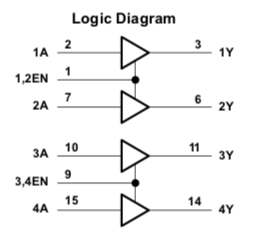
\includegraphics[width=0.4\linewidth]{l293d_logik}
	\caption[Logik des L293D-Mikrocontrollers, \url{http://www.ti.com/lit/ds/symlink/l293.pdf}, letzter Aufruf am 19.08.18, 12:51]{Logik des L293D-Mikrocontrollers}
	\label{fig:l293dlogik}
\end{figure}

Wie man in \autoref{fig:l293dlogik} sieht, ist der L293D eine doppelte H-Brücke. Genutzt werden nur drei Ein- und Ausgänge, der vierte bleibt frei. Die Pins $1,2EN$ sowie $3,4EN$ schalten nur die entsprechenden Transistoren ein. $V_{CC1}$ ist für die Spannungsversorgung des IC selbst und wird mit 5V beaufschlagt, an $V_{CC2}$ liegt die Versorgungsspannung für die Motoren, 14V, an. Die Anschlüsse $1-4A$ und $1-4Y$ stellen die Ein- und Ausgänge dar. In \autoref{fig:mikrocontroller-schaltung} auf \autopageref{fig:mikrocontroller-schaltung} wird die Schaltung dargestellt. Hierbei sei angemekrt, dass sich die GPIO-Pinbelegung am RaspberryPi durch das Layout auf der Latine noch geändert haben.
\begin{figure}[th]
	\centering
	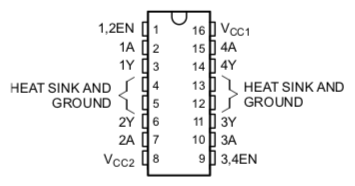
\includegraphics[width=0.6\linewidth]{l293d_pins}
	\caption[Pinbelegung des L293D-Mikrocontrollers, \url{http://www.ti.com/lit/ds/symlink/l293.pdf}, letzter Aufruf am 19.08.18, 12:51]{Pinbelegung des L293D-Mikrocontrollers}
	\label{fig:l293dpins}
\end{figure}

\subsection{Layout}
Wie in \autoref{fig:platine} zu sehen ist, befinden sich neben den ICs und den Eingangswiderständen noch die Anschlüsse für $Ground$ und $14V$ (ganz links, von unten nach oben) und eine 40-polige Brücke für die GPIO-Pins des RaspberryPi auf der Platine.\\\\
Die finale Pinbelegung am RaspberryPi ist wie folgt:

\begin{table}[htp] 
	\centering 
	\begin{tabular}{|c||c|c|c||c|}
		\hline 
		& 3,3V &  & 5V & alle $V_{CC1}$ und $xxEN$ \\ 
		\hline 
		& GPIO2 &  & 5V &  \\ 
		\hline 
		& GPIO3 &  & GND &  \\ 
		\hline 
		& GPIO4 &  & GPIO14 & Motor A Phase 3 \\ 
		\hline 
		GND 14V& GND &  & GPIO15 & Motor A Phase 1 \\ 
		\hline 
		& GPIO17 &  & GPIO18 & Motor A Phase 2 \\ 
		\hline 
		& GPIO27 &  & GND & GND $IC_{MotorA}$ \\ 
		\hline 
		& GPIO22 &  & GPIO23 &  \\ 
		\hline 
		& 3,3V &  & GPIO24 &  \\ 
		\hline 
		& GPIO10 &  & GND &  \\ 
		\hline 
		& GPIO9 &  & GPIO25 &  \\ 
		\hline 
		& GPIO11 &  & GPIO8 &  \\ 
		\hline 
		& GND &  & GPIO7 & Motor B Phase 3 \\ 
		\hline 
		& ID\_SD &  & ID\_SC &  \\ 
		\hline 
		& GPIO5 &  & GND &  \\ 
		\hline 
		& GPIO6 &  & GPIO12 & Motor B Phase 1 \\ 
		\hline 
		& GPIO13 &  & GND & GND $IC_{MotorB}$ \\ 
		\hline 
		Motor C Phase 2& GPIO19 &  & GPIO16 & Motor B Phase 2 \\ 
		\hline 
		Motor C Phase 1& GPIO26 &  & GPIO20 &  \\ 
		\hline 
		GND $IC_{MotorC}$& GND &  & GPIO21 & Motor C Phase 3 \\ 
		\hline 
	\end{tabular} 
	\caption{Pinbelegung am RaspberryPi} 
	\label{tab:pins}
\end{table}

\begin{figure} 
	\subfigure[Oberseite der Platine]{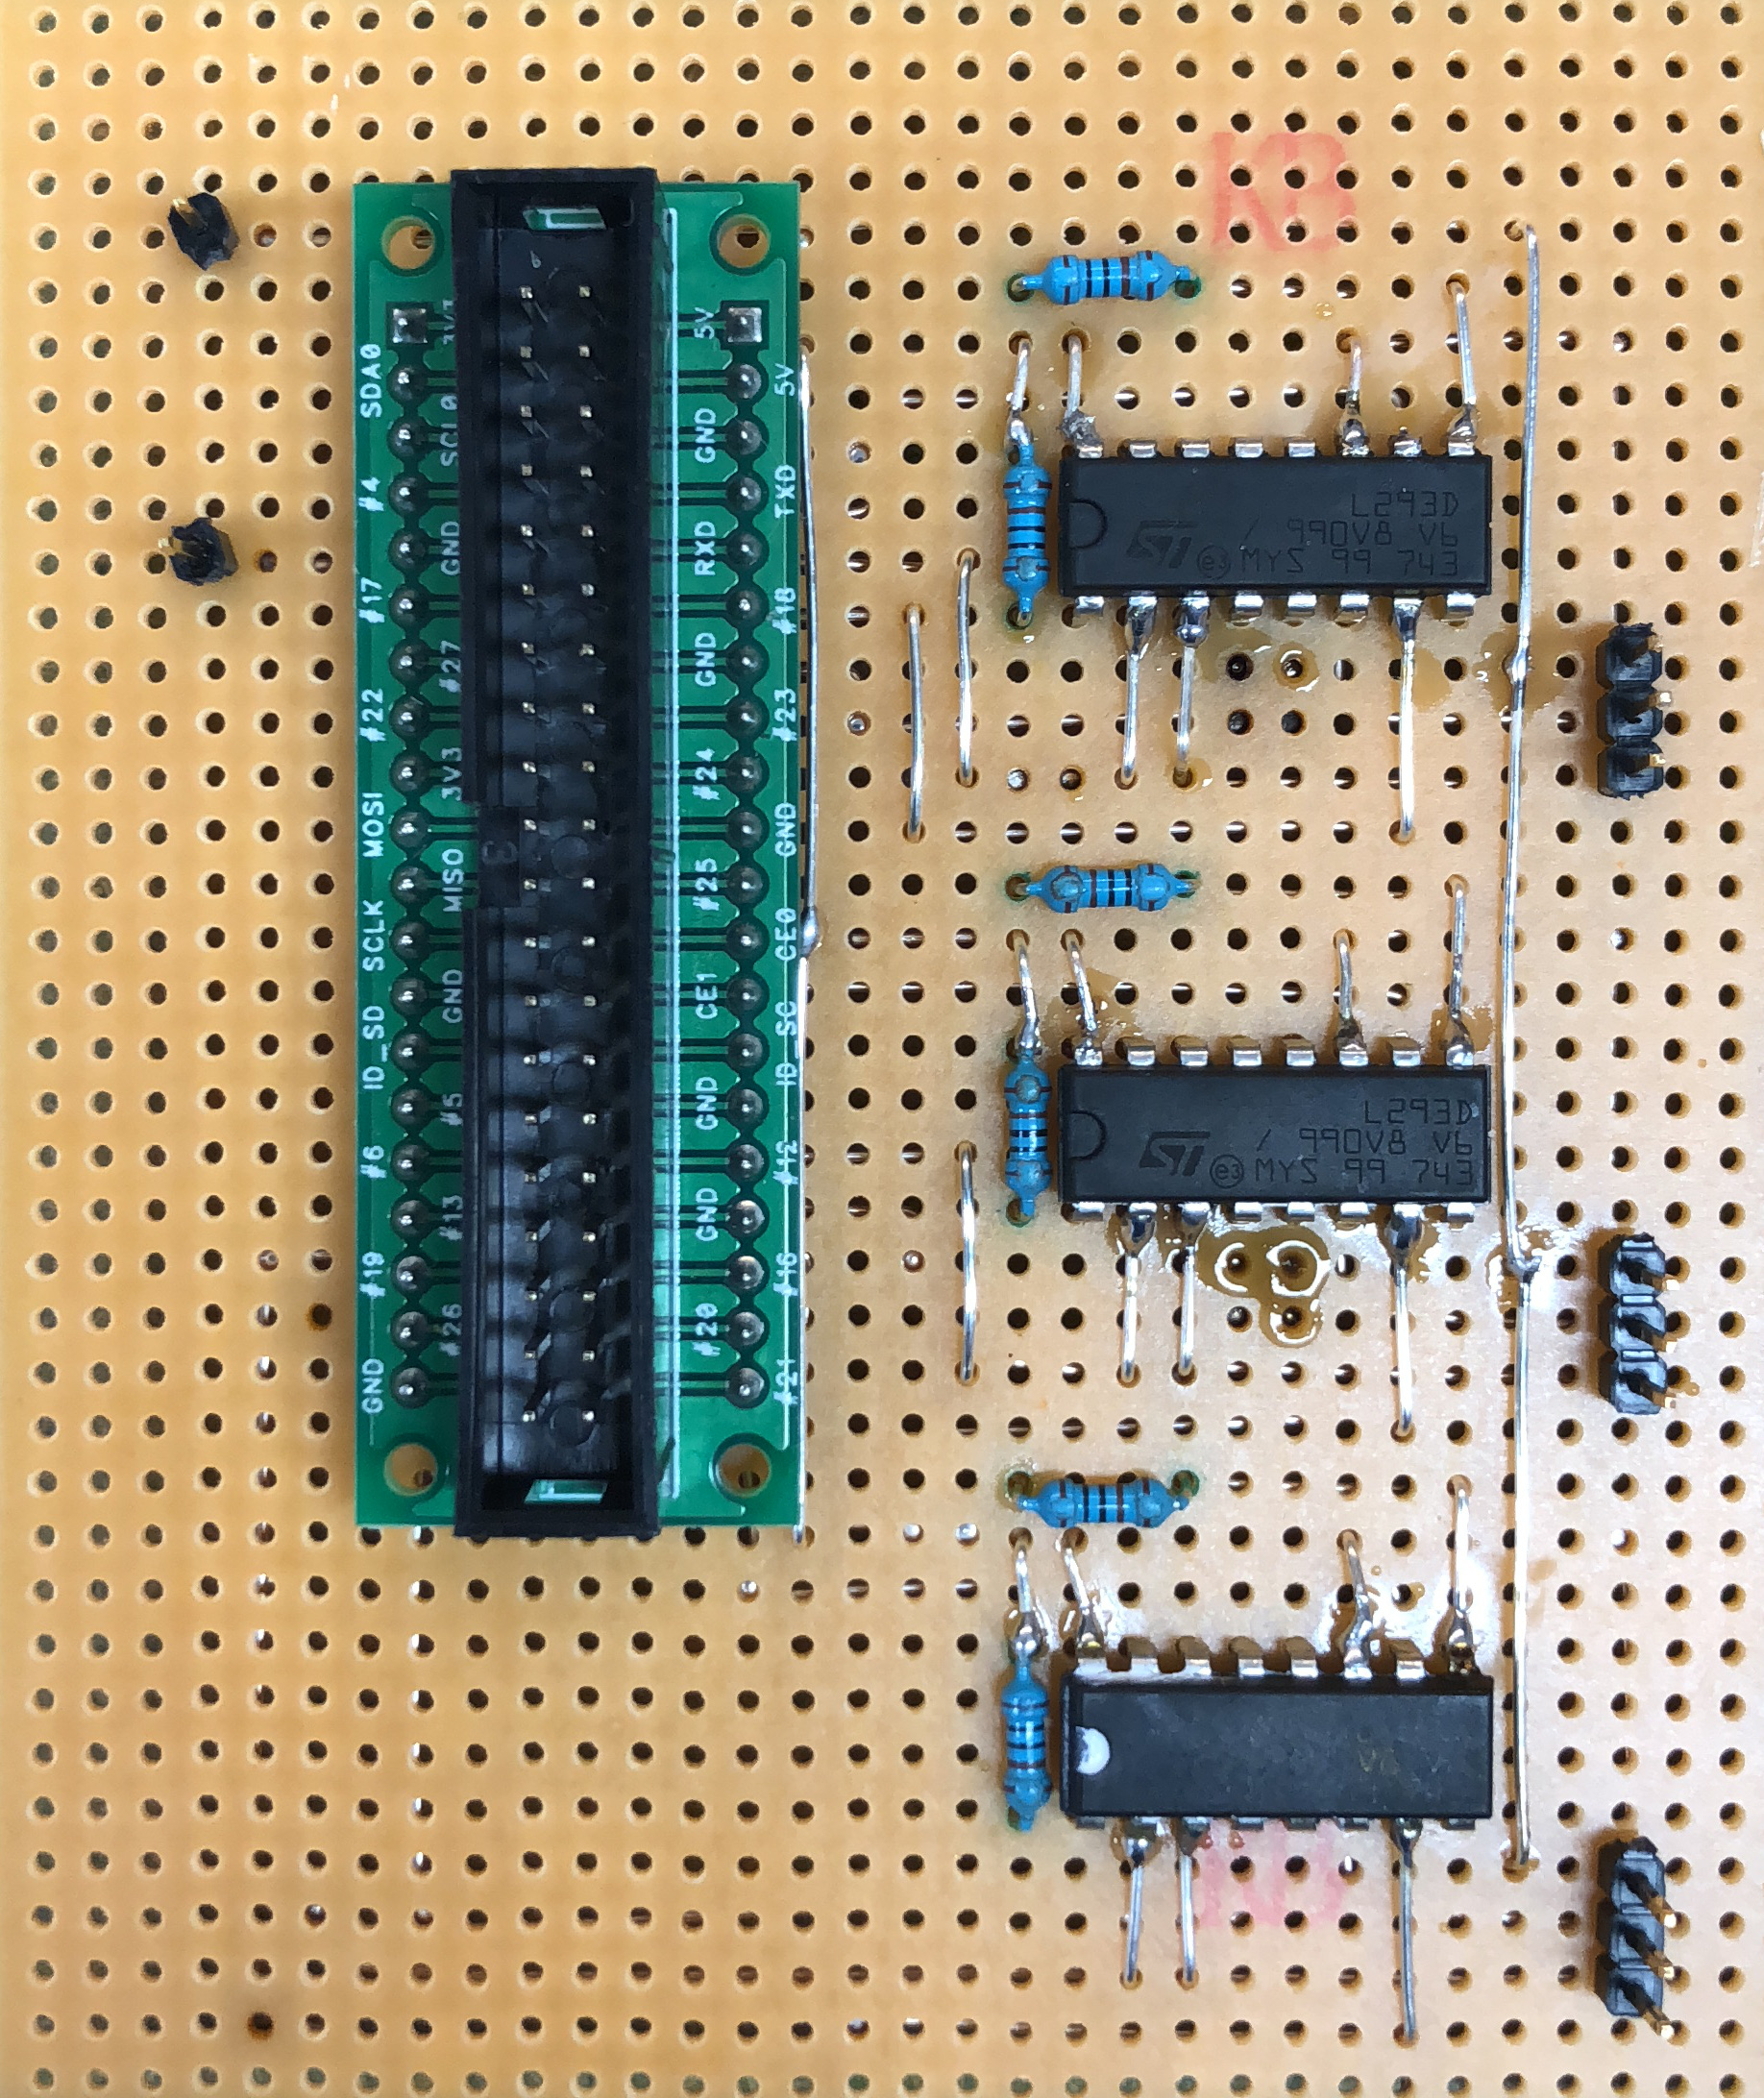
\includegraphics[width=0.49\textwidth]{platinevorn}} 
	\subfigure[Unterseite der Platine]{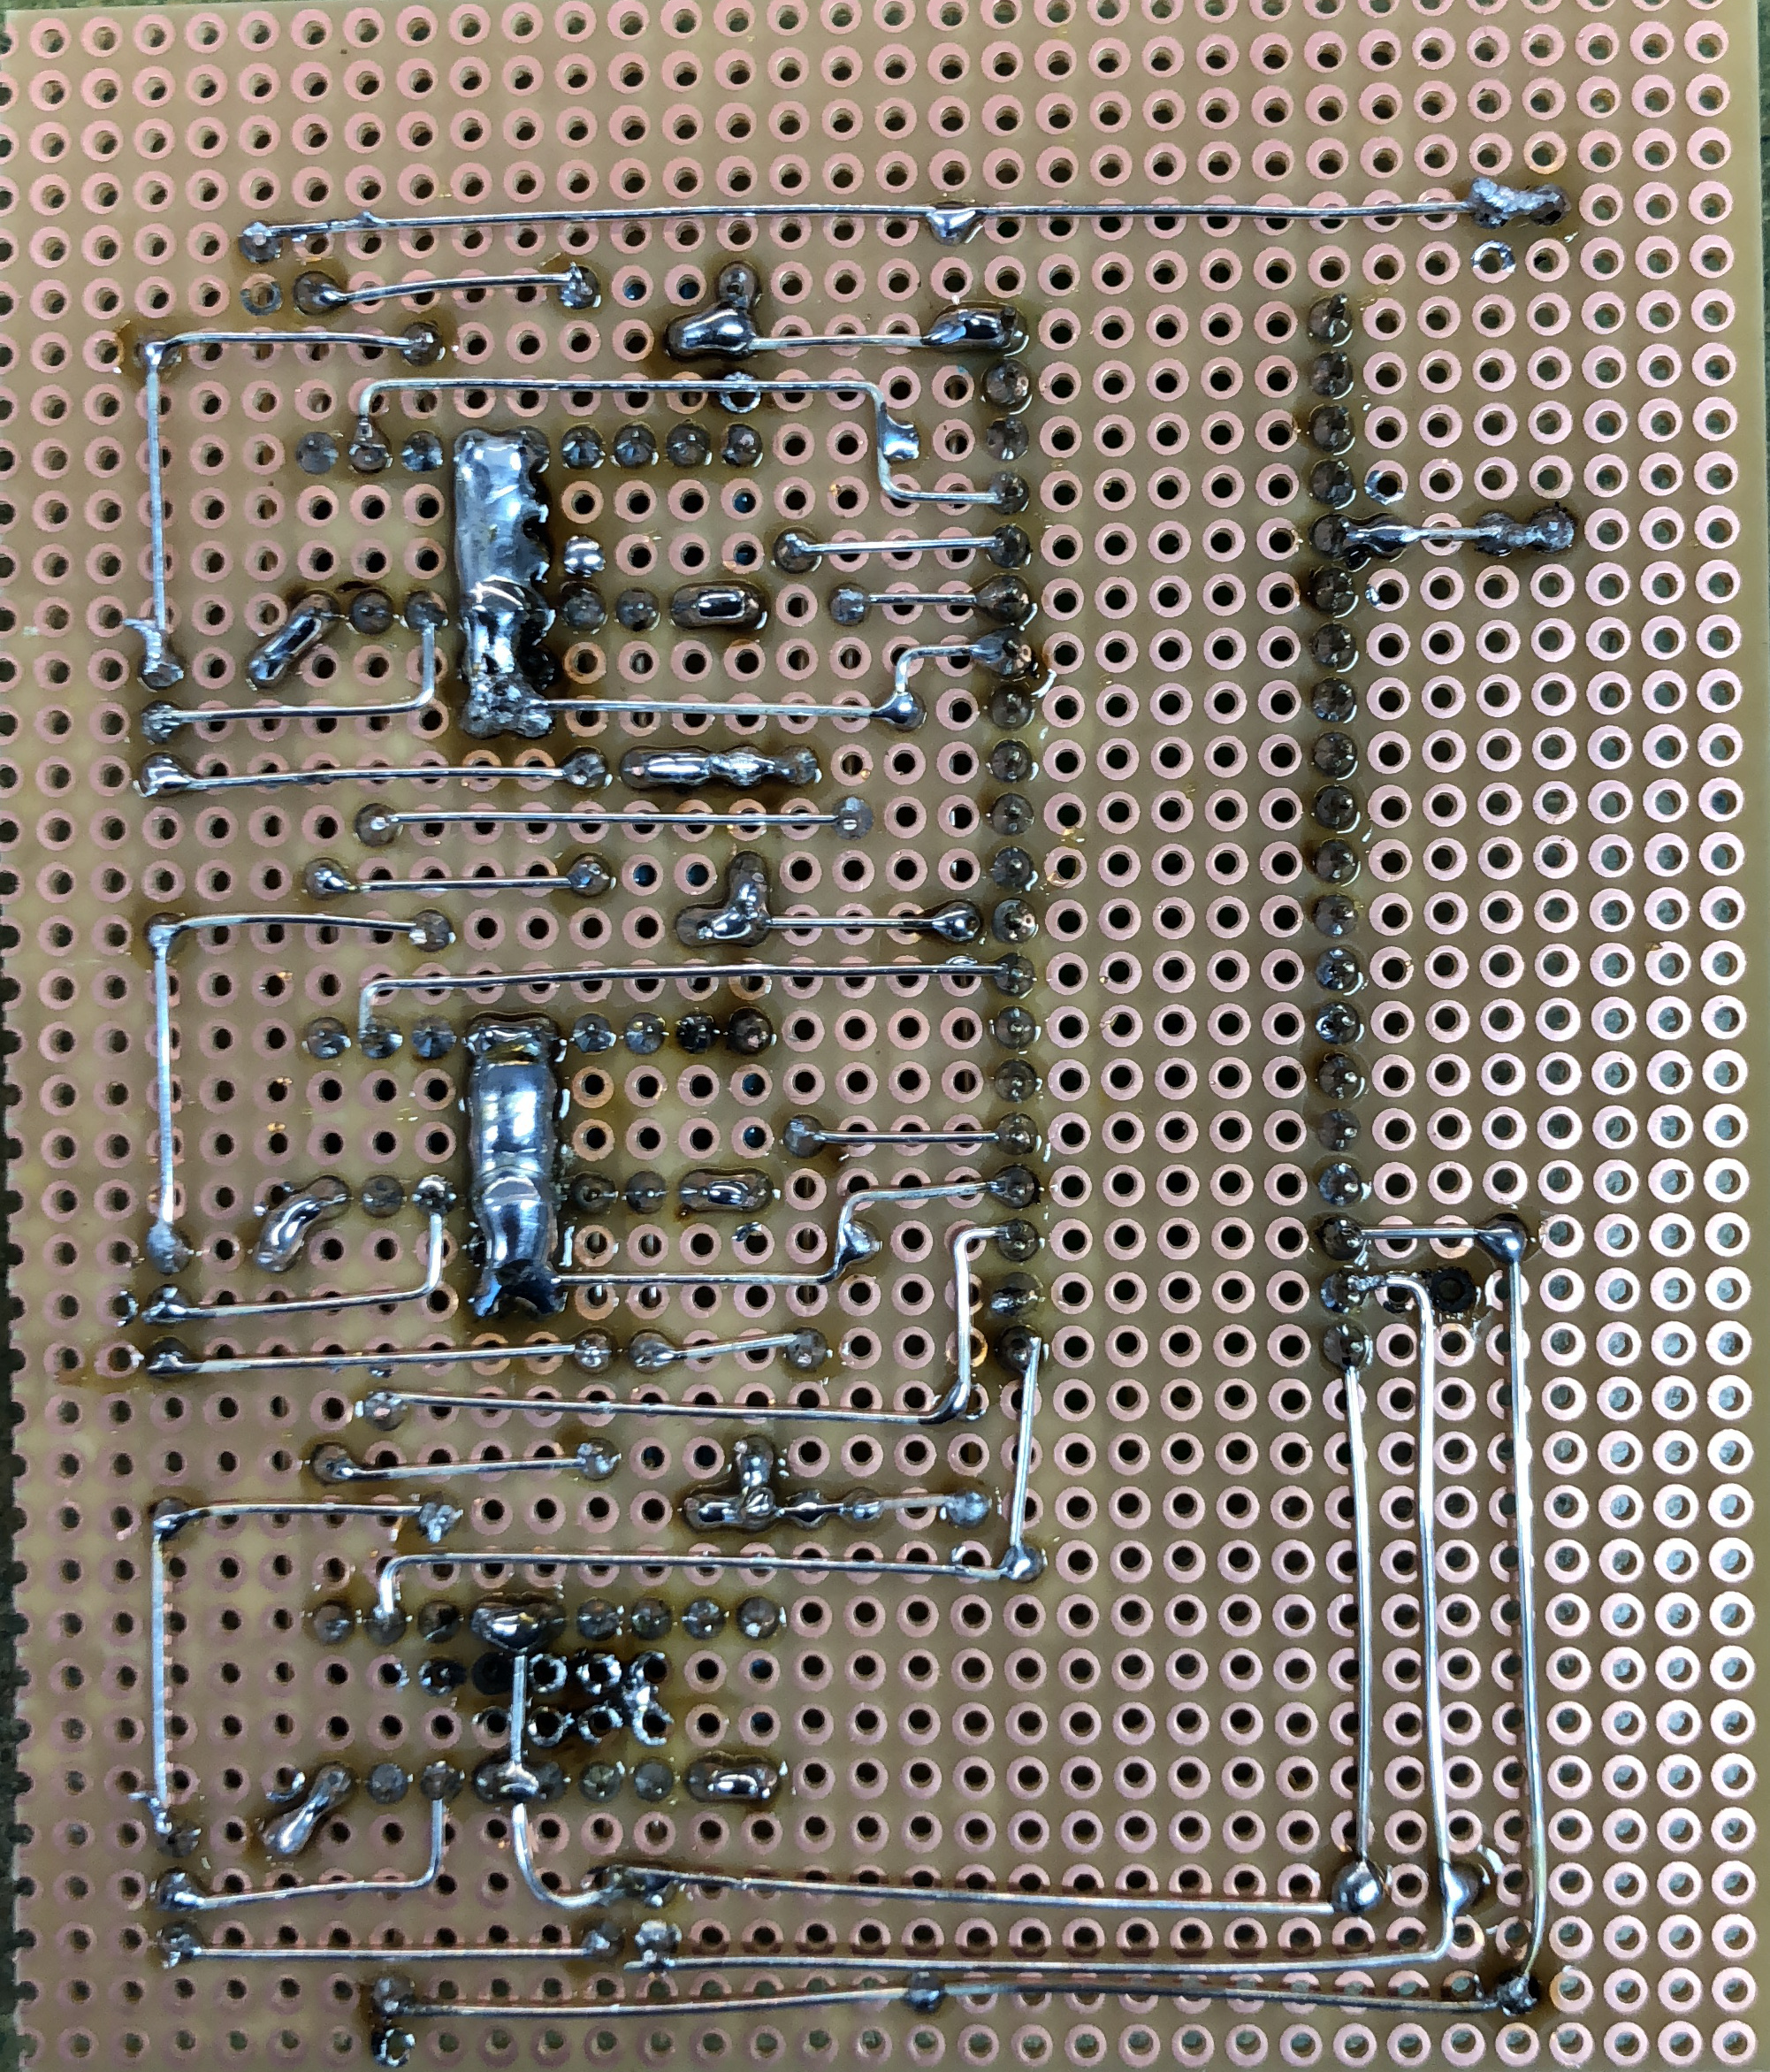
\includegraphics[width=0.49\textwidth]{platinehinten}} 
	\caption[Platine mit Brücke und Schaltung, aufgenommen von Erik Rother, 27.09.2018]{Platine mit Brücke und Schaltung} 
	\label{fig:platine}
\end{figure} 
\subsection{Ansteuerung der Motoren}
Geplant war die Ansteuerung der Motoren mit PWM-Signalen, um so die Phasenverschiebung der Phasen des Motors nutzen zu können und ihn beliebig langsam drehen zu lassen. Mangels Zeit haben wir dies nicht verwirklichen können. Die Motoren werden nun wie Schrittmotoren angesteuert. Das heißt es werden die 3 Phasen der Reihe nach an- und abgeschalten. Dadurch ergibt sich folgende Sequenz:
\begin{table}[htp] 
	\centering 
		\begin{tabular}{|c|c|c|c|}
			\hline
			0 & \textcolor{green}{an} & \textcolor{red}{aus} & \textcolor{red}{aus}  \\ 
			\hline 
			1 & \textcolor{green}{an} & \textcolor{green}{an} & \textcolor{red}{aus}  \\ 
			\hline 
			2 & \textcolor{red}{aus}  & \textcolor{green}{an} & \textcolor{red}{aus}  \\ 
			\hline 
			3 & \textcolor{red}{aus}  & \textcolor{green}{an} & \textcolor{green}{an} \\ 
			\hline 
			4 & \textcolor{red}{aus}  & \textcolor{red}{aus}  & \textcolor{green}{an} \\ 
			\hline 
			5 & \textcolor{green}{an} & \textcolor{red}{aus}  & \textcolor{green}{an} \\ 
			\hline
		\end{tabular} 
\caption{Sequenztabelle für einen Phasenumlauf} 
\label{tab:sequenz}
\end{table}

Wie aus \autoref{tab:sequenz} zu entnehmen ist, wird dadurch das Magnetfeld um jeweils einen halben Pol verschoben und der Motor dementsprechend bewegt. In Abschnitt \ref{berechnungSteps} wird die maximale Auflösung rechnerisch ermittelt.
\section{Aufbau des Gesamtsystems}
TO DO BILD \\ \\
Folgende Geräte und Bauteile wurden verwendet
\begin{itemize} 
\item Kamera: Guppy F - 146
\item Objektiv: Macro-CCD Lens 4x
\item Laptop mit FireWire-Schnittstelle
\item Raspberry Pi 2 Model B 
\item Bildschirm, Tastatur, Maus (einschließlich Kabel zum Anschließen an den Raspberry Pi)
\item Crossover-Kabel
\item Motoren: 3 mal BGM4108-130
\item Schaltung: Mikrocontroller: (L293D), Widerstände (1k Ohm), Brücken
\end{itemize}
TO DO vollständig und aktuell!! \\ \\
Die Position der Kamera ist durch ein Gestell mit drei Motoren variabel, wodurch ihr Winkel so eingestellt werden kann, dass sich Werkzeug und Werkstück optimal im Bildausschnitt befinden. Das Gestell kann sowohl an der Werkzeughalterung, als auch über der Werkstückaufnahme montiert werden. Im Rahmen unseres Projektes konnten wir die Montage TO DO realisieren.
Die Kamera ist über eine FireWire-Schnittstelle mit dem Laptop verbunden. Der Laptop speichert das Bildmaterial und stellt es per Ordnerfreigabe dem Raspberry Pi zur Verfügung. Bildschirm, Maus und Tastatur sind an dem Raspberry Pi angeschlossen, sodass der Benutzer mit Hilfe einer graphischen Oberfläche gewünschte Aktionen auswählen kann. Außerdem verfügt der Raspberry Pi über einen Algorithmus, der zusammenhängende Bereiche mit bestimmten Farbwerten erkennt, wodurch die Kamera automatisch dem Werkzeug folgen kann. (TO DO kann sie das?)

\section{Datenübertragung}
Die automatische Positionierung der Kamera setzt voraus, dass die Daten über den aktuellen Bildausschnitt bekannt sind. Die Kamera verfügt über eine FireWire-Schnittstelle. FireWire-Schnittstellen besitzen eine hohe Datendurchsatzrate, wodurch ein besonders schnelles Arbeiten möglich ist. FireWire 400 überträgt Datenströme und ist USB 2.0 daher besonders bei der Übertragung von kontinuierlichen Signalen zum Beispiel im Videobereich überlegen. Jedoch hat sich diese Schnittstelle auf dem Markt nicht durchgesetzt, weshalb viele aktuelle Geräte diese Schnittstelle gar nicht besitzen. USB bietet seit USB 3.0 eine so deutlich überlegene Übertragungsgeschwindigkeit, dass auch im Videobereich größere Datenraten übertragen werden können. \\ \\
Zur Verfügung steht uns ein Laptop der Firma Toschiba mit dem Betriebssystem Windows XP. Dieser bietet einen FireWire-Anschluss, sodass wir die Kamera anschließen können. Das Bildmaterial der Kamera wird mit einer Software von MatLab auf dem Laptop angezeigt und abgespeichert. Da dieser Laptop jedoch sehr langsam arbeitet, wird die weitere Verarbeitung der Bilddaten auf einen Raspberry Pi 2 Model B ausgelagert. \\ \\
Zur Übertragung der Bilddaten nutzen wir das Prinzip der Ordnerfreigabe. Das Betriebssystem Windows XP unterstützt Netzwerkfreigaben von sich aus, während der Raspberry Pi ein zusätzliches Programm für diese Funktion benötigt. Zum Einbinden der Windows-Freigabe nutzen wir das virtuelle Dateisystem \glqq cifs-vfs\grqq. Dazu wird das Paket \glqq cifs-utils\grqq auf dem Raspberry Pi installiert. Um den freigegebenen Ordner in das Dateisystem einzubinden nutzen wir den Befehl \glqq mount\grqq, wobei auch der Typ \glqq cifs\grqq und Angaben über den Ort des freigegebenen Ordners, sowie des Zielordners notwendig sind. Damit man den Ordner nicht bei jedem Neustart des Raspberry Pi's neu einbinden muss, hinterlegen wir alle Informationen für das Einbinden in der Konfigurations-Datei \glqq /etc/fstab\grqq. Nun werden beim Hochfahren des Raspberry Pi's alle Dateisysteme, die in \glqq /etc/fstab\grqq vermerkt sind und zu denen auch eine aktive Verbindung besteht, eingebunden. \\ \\
Für die Verbindung zwischen Laptop und Raspberry Pi gibt es mehrere Möglichkeiten. Wir haben uns mit den folgenden zwei Möglichkeiten beschäftigt. \\ \\
 Die erste Möglichkeit ist die Verbindung über das Netzwerk im LFM. Beide Geräte sind durch ein Ethernet-Kabel mit dem Netzwerk verbunden. Ein Vorteil ist, dass die Geräte auch so Zugang zum Internet haben. Der Laptop benötigt den Zugang zum Internet um die notwendigen Lizenzen für MatLab laden zu können. Der freigegebene Ordner kann nun in dem Netzwerk durch Angabe der IP-Adresse des Laptops im Netzwerk und Angabe des Freigabenamens gefunden werden. Dieser Ordner ist nun mit jedem Gerät in dem Netzwerk auffindbar, jedoch ist der Zugriff durch das Passwort des Benutzerkontos von dem Laptop geschützt. \\ \\
Die zweite Möglichkeit ist eine direkte Verbindung durch ein Crossover-Kabel. Diese Verbindung ist sicherer und die Daten können schneller übertragen werden. Jedoch ergibt sich das Problem, dass das Crossover-Kabel den gleichen Anschluss verwendet, wie das Ethernet-Kabel. So kann der Laptop nicht gleichzeitig mit dem Raspberry Pi verbunden sein und Zugang zum Internet haben. Den Internetzugang braucht er allerdings, um die MatLab-Lizenzen zu laden. So müsste zuerst das Ethernetkabel angeschlossen werde, sodass die Lizenzen laden können. Danach müsste man das Kabel entfernen und das Crossoverkabel anschließen, um die Verbindung zum Raspberry Pi herzustellen. Dies wäre nicht besonders anwenderfreundlich. Jedoch konnte diese Möglichkeit optimiert werden, indem durch einen Adapter ein zweiter Netzwerkanschluss an dem Laptop angebracht wurde. Dies ermöglicht Internetzugang mit einem Ethernet-Kabel und mit dem Crossoverkabel die Verbindung zum Raspberry Pi. Die IP-Adressen werden bei dieser Variante statisch gesetzt. So hat der Laptop die IP-Adresse \glqq 192.168.1.1\grqq und der Raspberry Pi die IP-Adresse  \glqq 192.168.1.2\grqq erhalten. Beiden wurde die gleiche Subnetzmaske  \glqq 255.255.0.0\grqq \\ übergeben. So kann der Ordner wieder durch die IP-Adresse des Laptops und den Freigabenamen gefunden und in das Dateisystem von dem Raspberry Pi einghängt werden. Mit dieser Variante wird nur ein LAN-Anschluss am Einsatzort des Systems benötigt und eine schnelle und sichere Datenübertragung ermöglicht, sodass wir uns für diese Variante entschieden haben. \\ \\
Durch die Arbeit mit mehreren Raspberry Pis benötigten wir die Einstellung, dass der Ordner für alle Benutzer freigegeben ist. Da der Laptop bei unserer Variante nun mit dem gesamten Netzwerk des Instituts verbunden ist, könnte man als eine zusätzliche Sicherheit (neben dem benötigten Passwort) die Ordnerfreigabe auf einen Benutzer beschränken. Dies müsste noch einmal durch einen Administrator des Laptops geschehen. 

\section{Hardwareentwicklung}
\subsection{Aufbau der Schaltung}
TO DO
\subsection{Steuerung der Motoren}
TO DO
\subsection{Konstruktion des Gestells}
TO DO

\section{Algorithmus zur Werkzeugerkennung}

Um die Werkzeugposition im aktuell ausgewählten Bild definieren zu können, haben wir uns überlegt, dies anhand von Pixelfarben zu realisieren. Denn man kann davon ausgehen, dass das Werkzeug in dem aufgenommen Bild größtenteils die gleiche Farbe hat oder nur kleine Farbabweichungen aufweist. Die Abweichungen können im Algorithmus kompensiert werden, je nach gegebenen Bedarf. \\  
Das von der Kamera aufgenommene Bild repräsentiert in Wirklichkeit nur einen ganz kleinen Ausschnitt, der keine weiteren größeren Objekte mit genau dieser Farbe enthalten dürfte. Aus diesem Grund nehmen wir an, dass das größte Objekt in dem Bild mit der ausgewählten Pixelfarbe dem Werkzeug entsprechen muss.

\subsection{Funktionsweise}
Um das Werkzeug in dem von der Kamera aufgenommen Bild zu finden, muss eine bestimmte Pixelfarbe ausgewählt werden.  Dem User werden bestimmte Farbe schon in der GUI vorgegeben, die der Werkzeugfarbe entsprechen könnten. Des Weiteren kann er jedoch auch eine Farbe selber auswählen, in dem er diese anhand von RGB-Werten eingibt oder mithilfe von einem Klick in das aktuell ausgewählte Bild die gewünschte Farbe definiert. Nun durchsucht der Algorithmus das komplette Bild nach dieser Farbe. Zuvor kann noch entschieden werden, ob nur nach genau dieser Farbe gesucht werden soll oder man einen gewissen Wertebereich zulassen möchte, den man dann selber angeben kann. Beim Durchsuchen des Bildes wird jede Zeile von links nach rechts durchsucht und es werden sogenannte Segmente gebildet, wenn die übergebene Farbe gefunden wurde. Ein Segment besteht dabei aus einem Start- sowie einem Endpunkt und der dazugehörigen Y-Koordinate. Wenn das Segment die angeklickte Position im Bild enthält, wird noch ein Merker gesetzt um dieses Segment als Werkzeug zu markieren. Im nächsten Schritt werden nun die Segmente, die zusammenhängen, miteinander verbunden. Segmente gehören zusammen wenn sie über- oder untereinander liegen und sich mit mindestens einem Pixel überlappen. Aus diesen zusammenhängenden Segmenten werden dann Bereiche gebildet. Wenn bei einem Segment aus diesem Bereich der Merker gesetzt ist, wird auch für den ganzen Bereich der Merker gesetzt, denn dann ist der ganze Bereich das Werkzeug. Wurde jedoch die Farbe durch eine Eingabe definiert oder eine der vorgegeben Farben ausgewählt, so werden die verschiedenen Bereiche durchlaufen und der mit der größten Anzahl an Pixeln, wird als Werkzeug definiert. Denn es ist davon auszugehen, dass es in dem kleinen Bildausschnitt nicht noch ein weiteres Objekt gibt, welches genau die gleiche Farbe hat.


\section{Graphische Oberfläche}
In der GUI werden dem User verschiedene Möglichkeiten geboten, die Motoren einfach ansteuern zu können oder sogar automatisch an eine gewünschte Position verfahren zu lassen.  Des Weiteren ist die graphische Oberfläche dazu da, um Berechnungen, die im Hintergrund ausgeführt werden, zu starten und deren Ergebnisse wiederum an andere Funktionen weiterzuleiten, die die zuvor berechneten Werte als Eingabe benötigen.
Eine weiter wichtige Aufgabe ist das Anzeigen des aktuell aufgenommen Bildes der Kamera, welches das Werkzeug sowie Werkstück enthält. Jedoch besteht nicht nur die Möglichkeit sich das aktuelle Bild anzusehen, man kann sich auch noch zuvor aufgenommen Bilder anschauen, um Einstellungen zu vergleichen oder um doch mit früheren Positionen weiterarbeiten zu können.

\subsection{Berechnungen}
\subsubsection{Steps}
\label{berechnungSteps}
Steps pro Umdrehung: \\
$22*3 = 66 $\\
Winkel pro Step: \\
$360/66 = 60/11 = 5.4545$\\
\subsection{Abstand und Winkel}
Das Gestell ist mit drei Motoren ausgestattet, um die Kamera richtig zu positionieren. Motor A bewegt die Kamera in aus der Draufsicht betrachtet in einer Kreisbahn, sodass die x-Position des Bildausschnittes verändert werden kann. Durch diese Kreisbahn ändert sich jedoch auch der Abstand von Kamera zu Werkstück. Um den genauen Abstand einzustellen wird die Kamera durch Motor B vor und zurück geschwenkt. Auch dies geschieht auf einer Kreisbahn. So verändert sich mit dem Abstand zum Werkstück auch die Höhe der Kamera. Mit Motor C kann die Kamera hoch und runter gekippt werden, wodurch die zuvor entstandene Höhendifferenz wieder ausgeglichen werden kann. Außerdem wird durch diesen Motor die y-Position des Bildausschnittes eingestellt.

\begin{figure}[htbp]
\centering 
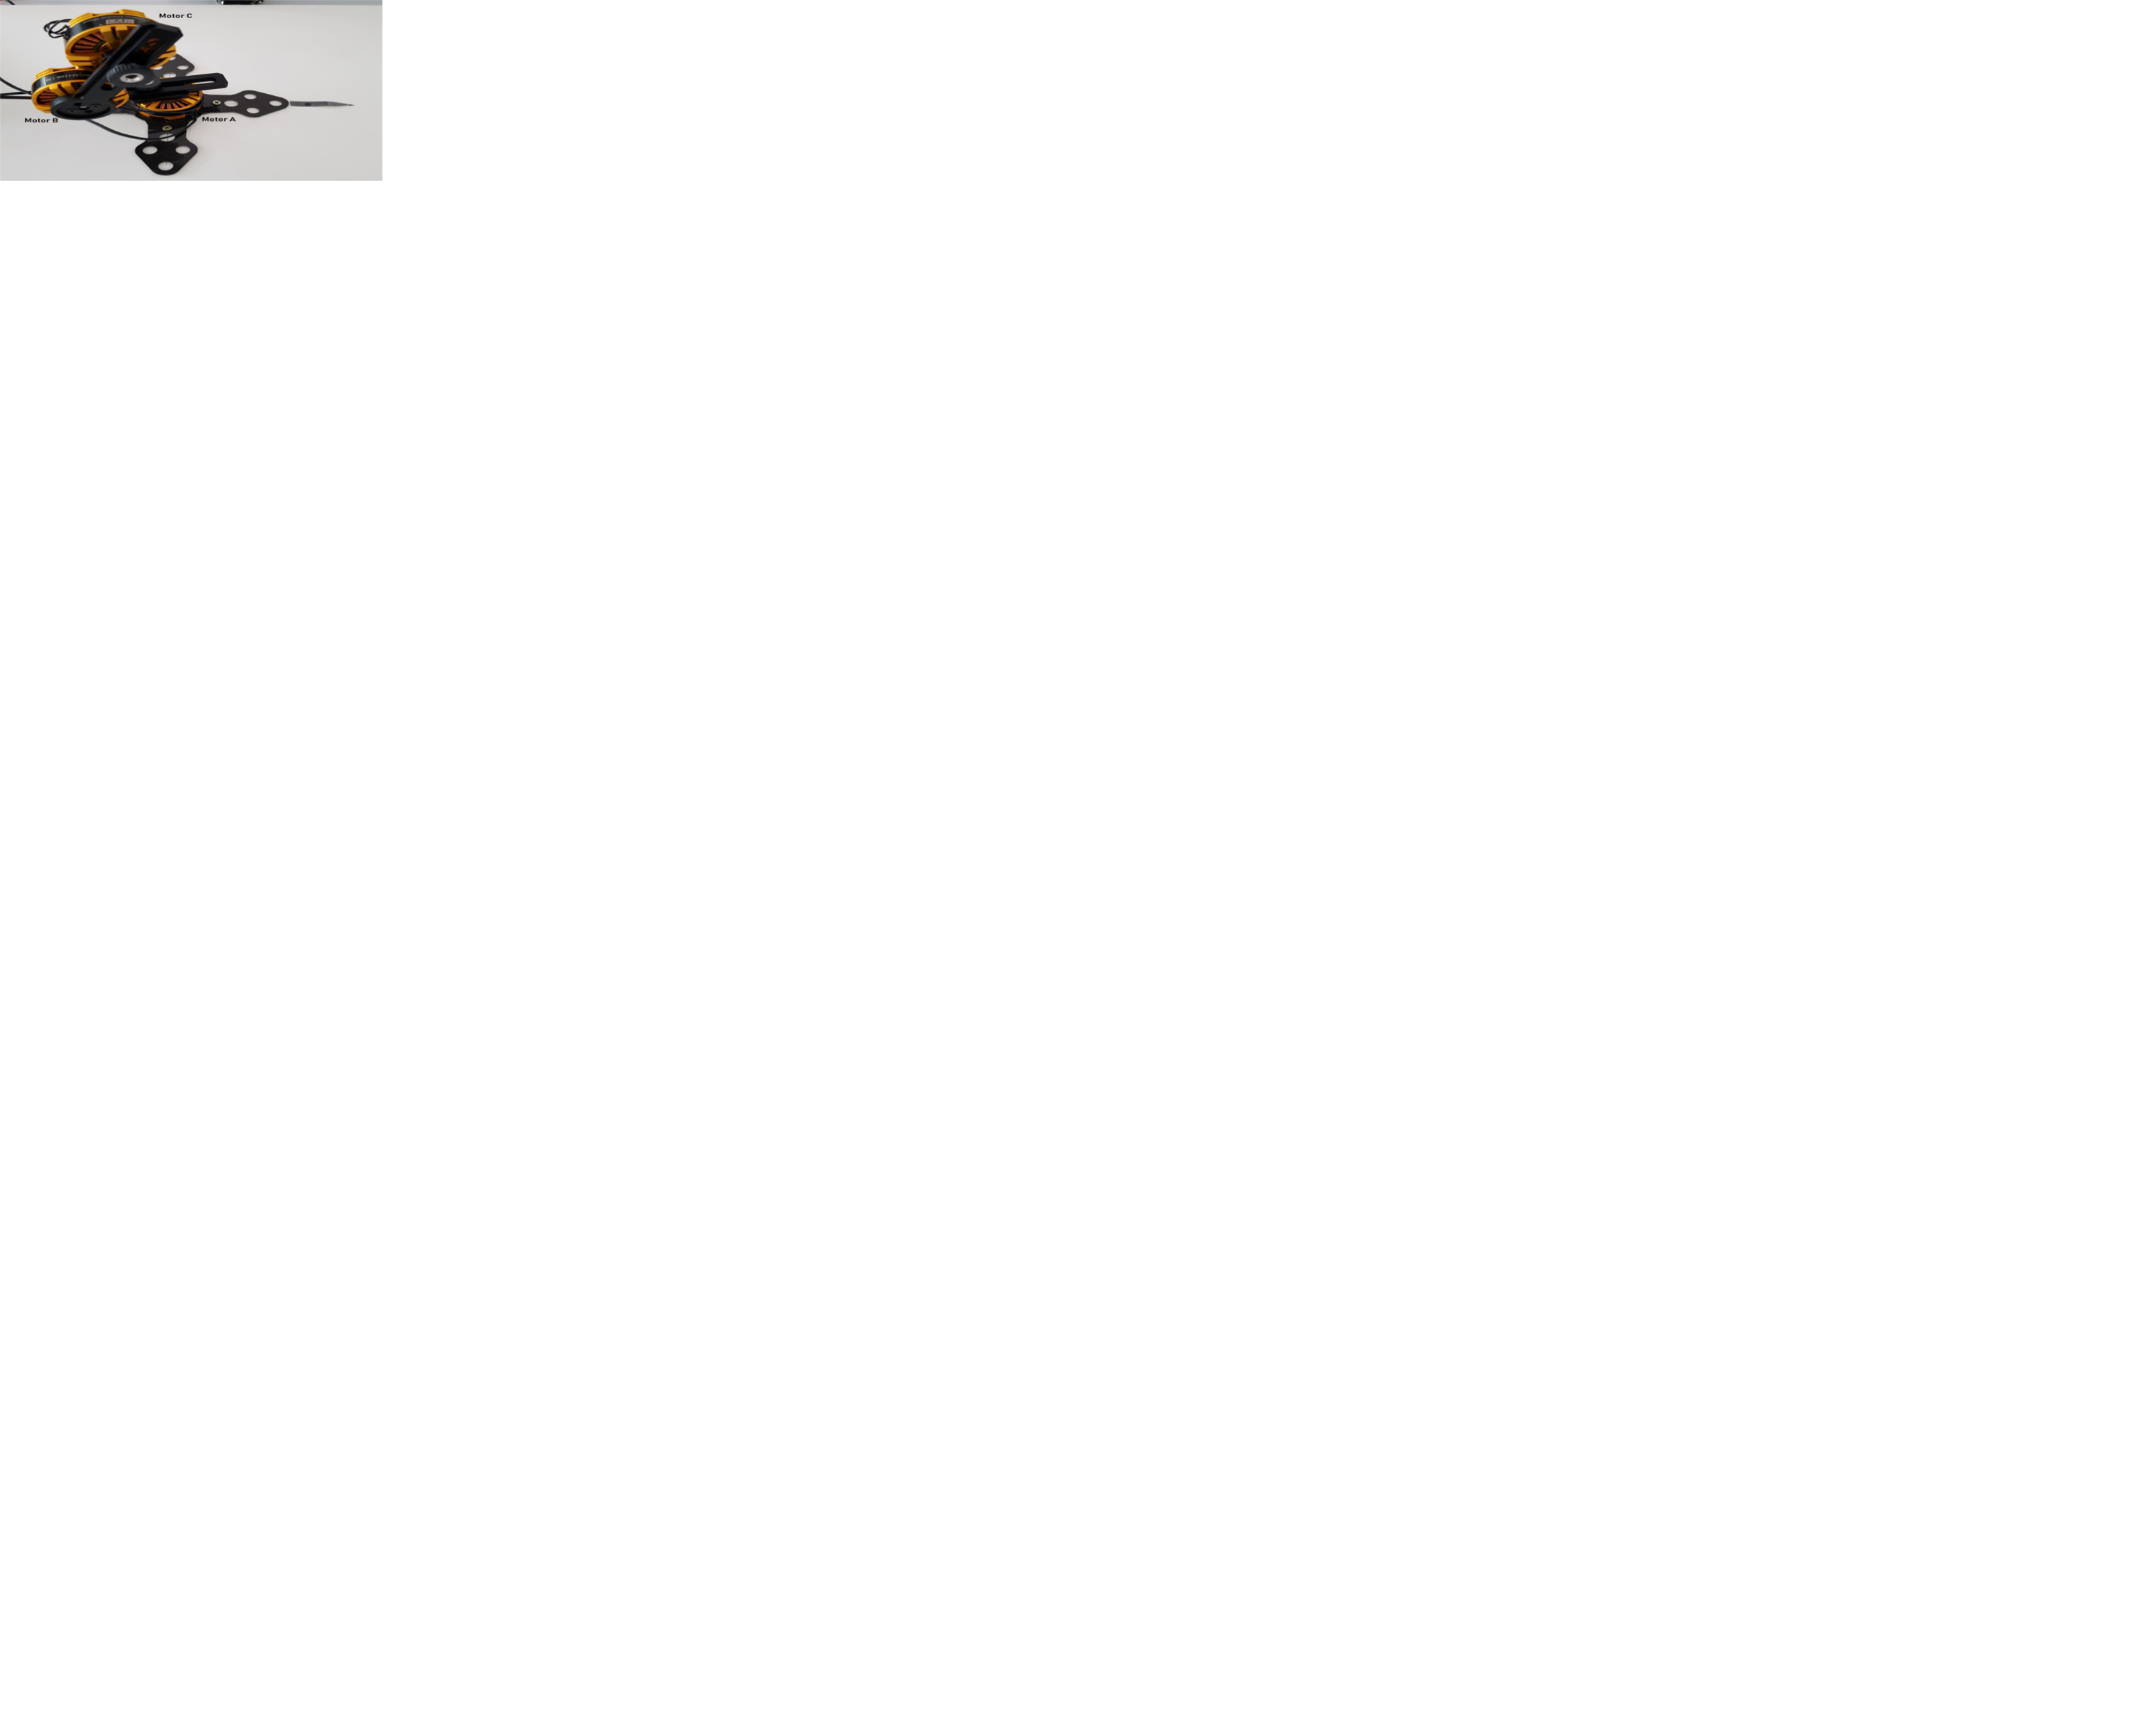
\includegraphics[width=0.5\textwidth]{Motoren.PNG}
\caption{Gestell mit den drei Motoren}
\label{fig:Bild6}
\end{figure}
\break
In Abbildung 7 ist die Bahn, entlang der sich die Kamera durch Motor A bewegt, in der Draufsicht zu sehen. Ausgehend von der Position mittig auf dem Halbkreis kann die Kamera zu beiden Seiten geschwenkt werden. Während sie mittig den größten Abstand zum Werkstück hat, wird der Abstand beim Schwenken zu den Seiten geringer. Zu dem Abstand zwischen Motor A und Werkstück wird dann $cos(\alpha) * Radius A$ gerechnet. Der Cosinus beträgt bei 0$^\circ$ 1, dies entspricht genau der Position mittig auf dem Halbkreis, da in dem Fall der Abstand mit Abstand zwischen Motor A und Werkstück + Radius A am größten ist. 
\begin{figure}[htbp]
\centering 
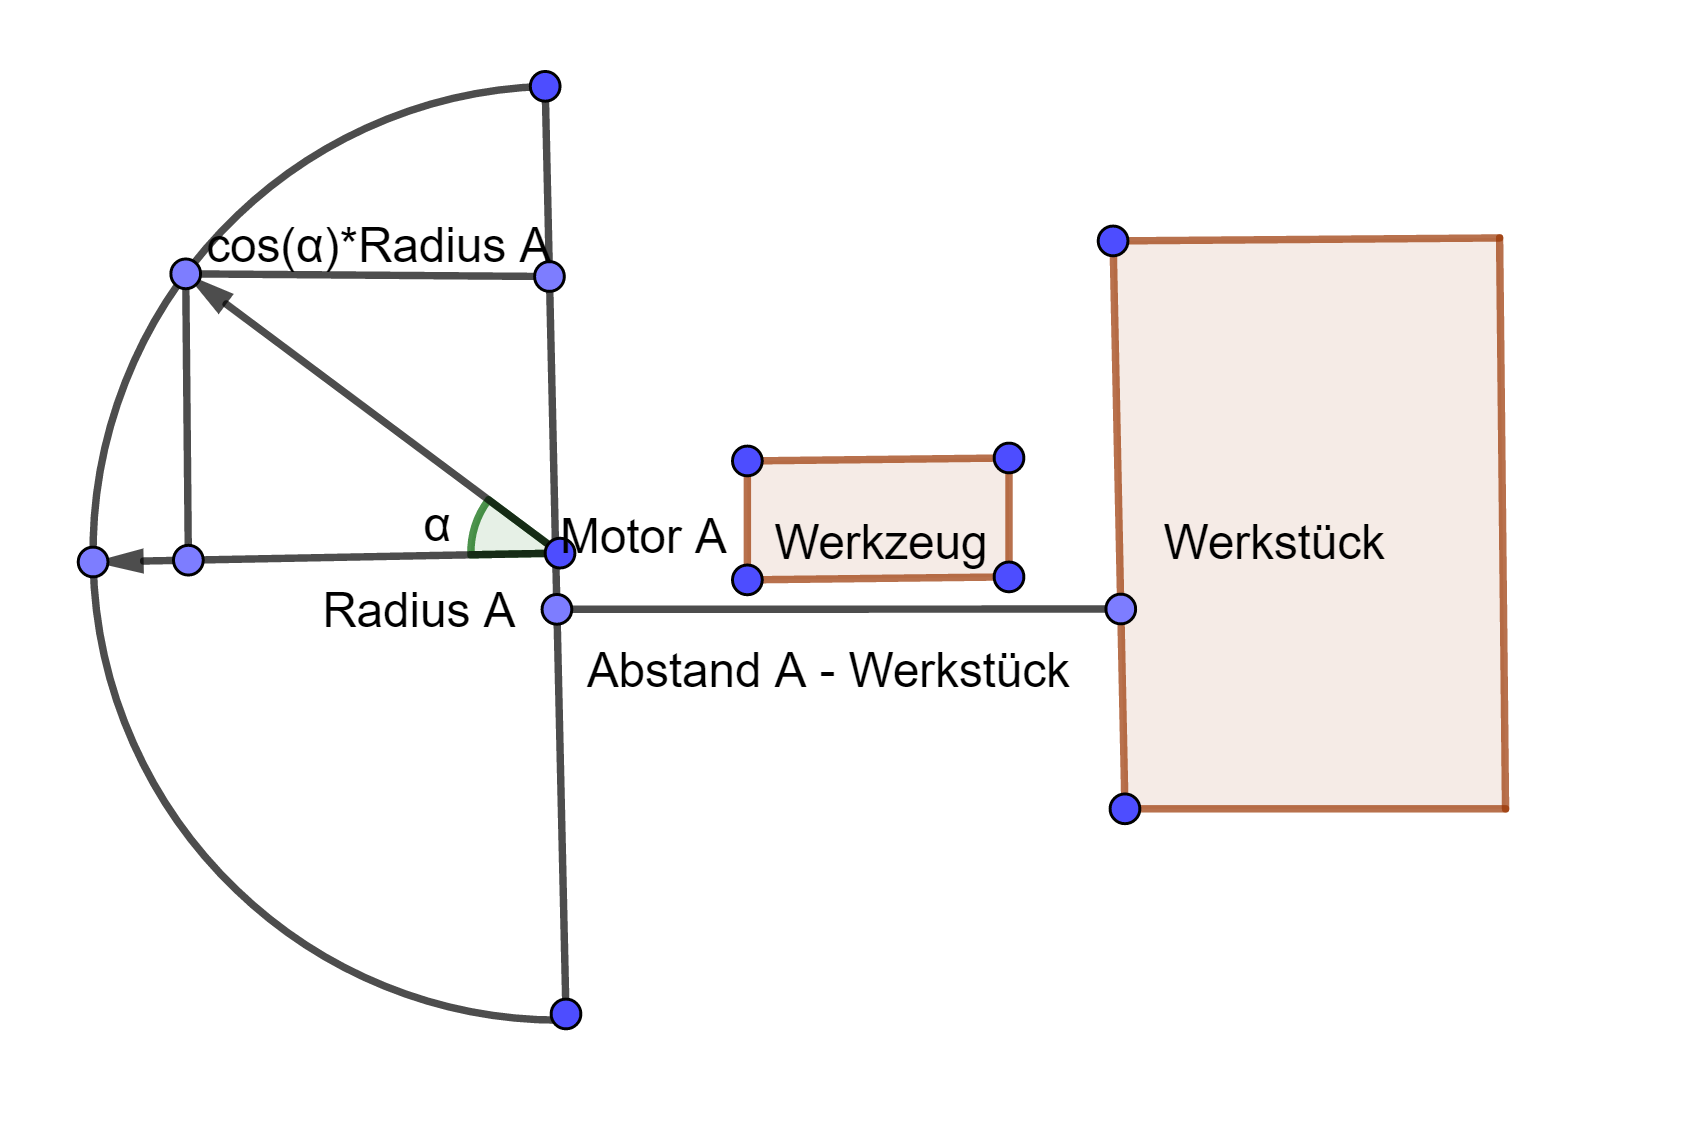
\includegraphics[width=0.8\textwidth]{Motor_A.PNG}
\caption{Positionsänderung der Kamera durch Motor A}
\label{fig:Bild7}
\end{figure}
\break
In Abbildung 8 erkennt man nun die Bahn, entlang der sich die Kamera durch Motor B bewegt aus seitlicher Ansicht. Der Abstand zum Werkstück soll hier korrigiert werden. Die Kamera kann auf der Kreisbahn näher zum Werkstück hingeführt werden. Von dem ursprünglichen Abstand wird dann $Sin(\beta)*Radius B$ subtrahiert, da der Abstand kleiner wird. Schwenkt man die Kamera nach hinten wird der genannte Therm addiert, da sich der Abstand vergrößert. Jedoch bewegt sich die Kamera entlang dieser Kreisbahn auch in ihrer Höhe. Die Höhe ändert sich um den Therm $Radius B - Cos(\beta) *Radius B$. Sowohl dieser Höhenunterschied muss durch den Motor C ausgeglichen werden, als auch der Winkel, den Motor B verstellt. Wird die Kamera beispielsweise durch Motor B etwas nach unten gekippt, neigt Motor C die Kamera wieder um dieses Winkel nach oben. Außerdem wird die Höhendifferenz auf dem Bildausschnitt berechnet und die Kamera wird so weit nach oben geneigt, bis sie wieder den richtigen Bildausschnitt zeigt.
\begin{figure}[htbp]
\centering 
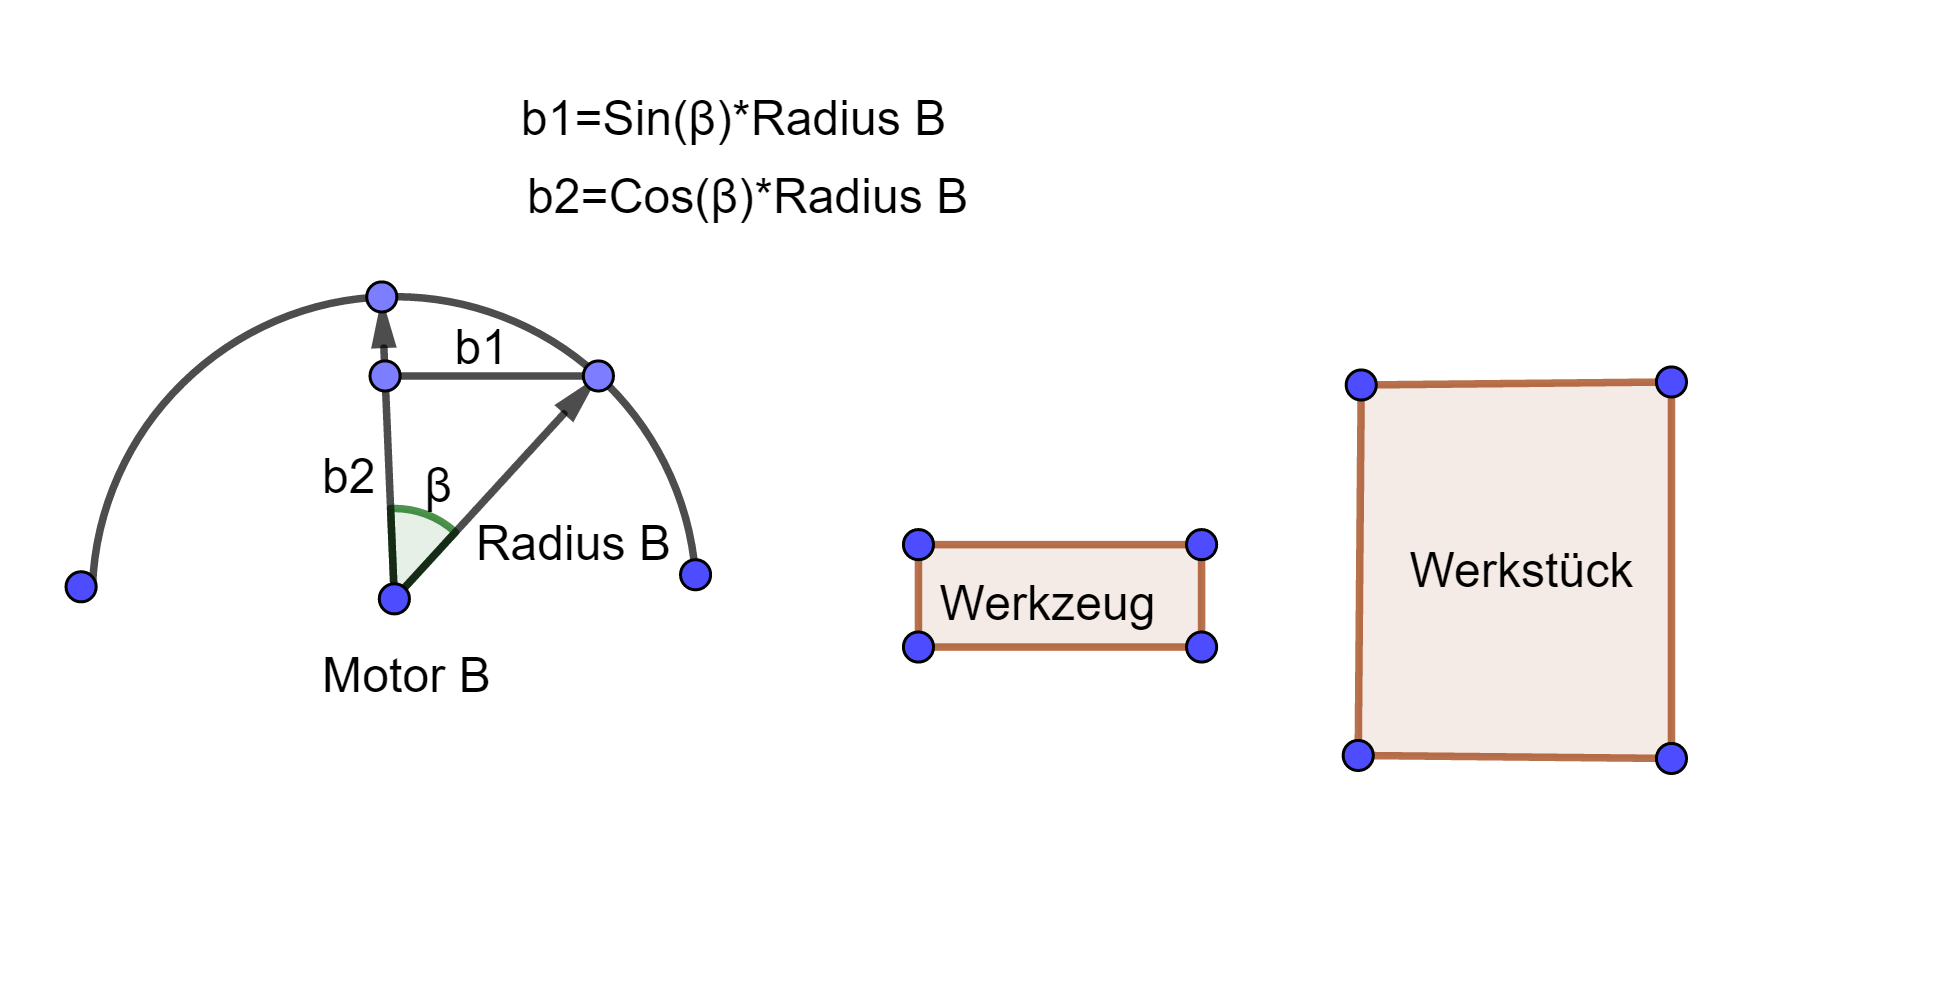
\includegraphics[width=0.8\textwidth]{Motor_B.PNG}
\caption{Positionsänderung der Kamera durch Motor B}
\label{fig:Bild8}
\end{figure}
\break
Bei den Berechnungen wurde die Annahme getroffen, dass die Distanzänderung, die nur durch den Winkel des Motors C entsteht vernachlässigt werden kann. Es ist anzunehmen, dass die Winkeländerungen von Motor C im Vergleich zu dem Abstand zum Werkstück so gering sind, dass sich die Distanz nur minimal ändert. Sollte es trotzdem zu unscharfen Bildern kommen, kann man die Motorpositionen durch ein iteratives Verfahren optimieren. In diesem Verfahren würde die Abstandsdifferenz zwischen angenommenem Abstand und wahrem Abstand mit Hilfe von Cosinus berechnet. Der Abstand würde durch Motor B angepasst und anschließend würde der Winkel von Motor C entsprechend den Änderungen durch Motor B wieder angepasst. Durch mehrfaches Ausführen dieser Schritte könnte man den Abstand optimieren. Jedoch haben wir uns gegen eine solche Optimierung entschieden, da zunächst die grundlegenden Funktionen unserer Positionierung im Vordergrund stehen sollten. 

\section{Bedienungsanleitung}
TO DO (finale Version)
\renewcommand{\labelitemi}{$\bullet$}
\renewcommand{\labelitemii}{$\bullet$}
\begin{itemize} 
\item Kamera einrichten...
\item Laptop einschalten, Benutzer: Doer-se-proj anmelden
\item Laptop via Ethernetkabel mit Netzwerk verbinden
\item Adapter für weiteren Netzwerkanschluss an Laptop anschließen und Laptop über diesen Adapter mit Raspberry Pi via Crossover-Kabel verbinden
\item Bildschirm, Tastatur und Maus an Raspberry Pi anschließen und diesen mit Strom versorgen
\item Es ist zu beachten, dass Laptop und Raspberry Pi verbunden sind bevor der Raspberry Pi hochfährt
\item Bild aufnehmen\\
Das Lifebild von der Kamera wird mithilfe von MatLab angezeigt. Damit man sich die Echtzeitübertragung der Kamera angucken kann, muss nur das Skript \glqq save\_image.m\grqq{} ausgeführt werden. Nun hat der Nutzer die Möglichkeit das aktuelle Bild zu speichern, indem er einen Impuls an das Programm sendet, dadurch, dass er  die Taste \glqq s\grqq{} drückt. Somit wird das Bild, in dem Ordner auf den auch der Rasperry Pi zugreifen kann, gespeichert und als Dateiname wird der dazugehörige Zeitstempel verwendet. Anschließend läuft das Programm weiter, damit noch weitere Aufnahmen gemacht werden können. Des Weiteren ist es auch möglich, das Programm mittels einer Tastatureingabe (\glqq q\grqq{}) zu beenden.
\item GUI 
\begin{itemize}
\item letzte Position\\
Die Funktion \glqq letzte Position\grqq{} ermöglicht ein schnelles Positionieren der Motoren. Die Motoren nehmen die Position ein, die sie bei der letzten Kameraaufnahme hatten.
\item Zielfahrt\\
Mit der \glqq Zielfahrt\grqq{} wurde die Möglichkeit gegeben, die neue Kameraposition in Bezug auf  das aktuelle Bild neu zu bestimmen. Der Nutzer muss nur einfach in das Bild an die Stelle klicken, die als nächstes im Mittelpunkt des Bildes zu sehen sein soll. Nach dem dies geschehen ist, werden die neuen Motorpositionen berechnet und die Motoren werden neu positioniert.
\item Tracking\\
Um den Werkzeugmittelpunkt auch in der Mitte des Bildes zu haben, kann die Methode Tracking verwendet werden. Die Methode braucht nur eine Pixelfarbe, anhand dieser wird dann das Werkzeug erkannt und in dem Bildausschnitt definiert. Die Pixelfarbe kann aber auch in einem Wertebereich liegen, dann muss der Nutzer nur noch diesen Wertebereich festlegen oder sagen, dass die Methode nur genau nach dieser Farbe suchen soll. Anschließend wird dann das Werkzeug mittels dem zuvor beschriebenen Algorithmus aus dem Bildausschnitt heraus gefiltert und dessen Mittelpunkt bestimmt. Dabei entspricht der ermittelte Werkzeugmittelpunkt nicht dem echten Mittelpunkt, sondern bezieht sich nur auf den Werkzeugausschnitt, der in dem Bild zu sehen ist.  Nun  wird noch der Werkzeugmitte als neuer Mittelpunkt des Bildes gesetzt und die Motoren verfahren dementsprechend.
\item Koordination\\
Der Reiter Koordination beinhaltet zwei ähnliche Funktionen. Bei der einen kann der Anwender die x- und z-Koordinate von dem aktuellen Bild angeben, an die die Kamera fahren soll. Mit der anderen kann man die Motorposition explizit angeben, dabei ist zu beachten, dass der eingegebene Wert Motorschritten entspricht und nicht einem Winkel.
Bei beiden Funktionen ist es noch möglich die Zeitverzögerung der Schritte einzustellen.
\item Navigation\\
Navigation ist ein einfaches Tool, um die Motoren steuern zu können. Mit den Buttons kann man ganz einfach die Motoren nach oben (-y), unten (+y),  links (-x) und rechts (+x) fahren lassenausgehend von der aktuellen Position der Motoren. Dabei steht einmal Drücken (Button anklicken) für einen Schritt in die jeweilige Richtung der entsprechenden Motoren.
Es werden dem User noch zwei zusätzliche Funktionen geboten, zum einen kann er entscheiden, wie schnell die Schritte ausgeführt werden sollen. Dafür stehen ihm zwei verschiedene Auswahlmöglichkeiten zur Verfügung. Des Weiteren kann er den Motoren das Signal geben, dass diese genau auf die andere Seite fahren sollen. Jedoch bevor die Motoren ihre neue Position einnehmen, wird noch einmal zur Absicherung abgefragt, ob die Motoren dort hinfahren können, nicht dass sich ein anderes Objekt in der Fahrbahn befindet. Die zuletzt genannte Funktion wurde eingebaut, falls ein Gegenstand, zum Beispiel das Werkzeug selbst, den Blick auf den Abstand zwischen Werkzeug und zu bearbeitender Oberfläche versperrt.
\item Bilder\\ 
Über den Button Bilder kommt man zu einer Seite, auf der verschiedene Bilder, die vorher mit der Kamera aufgenommen wurden, angezeigt werden. Es werden die neun zuletzt aufgenommen Bilder dargestellt, damit auch ältere Bilder wieder verwendet werden können, sowie die dazugehörige Kameraeinstellung. Um eines dieser Bilder auszuwählen, muss dieses einfach nur angeklickt werden. Mittels des Anklickens werden die Bilder der Funktionen letzte Position, Automation, Tracking, Koordination und  Navigation an das neu ausgewählte Bild angepasst sowie die dazu gehörigen Motoreneinstellungen geladen.
\item Bilder neu laden\\
Um zwischendurch die Bilder aktualisieren zu können, kann der User in der Linkensidebar den Button \glqq Bilder neu laden\grqq{} anklicken. Somit wird eine Funktion ausgelöst, die sich aus dem \glqq shared-Ordner\grqq{} alle Dateien holt und die neun neusten Bilder herausfiltertet. Anschließend werden die neuen Bilder in die GUI geladen und unter dem Reiter Bilder angezeigt
\item Abstandseingabe\\ 
Weil es nicht möglich ist, die Kamera immer genau an der selben Position  im Maschinenraum zu befestigen genau, und dies noch auf einen Millimeter genau, kann der genaue Abstand zwischen Motor a und dem Werkstück per Hand an die graphische Oberfläche übergeben werden. Somit können alle folgenden Berechnungen auf genau diesen Aufbau bezogen werden. Des Weiteren ermöglicht diese Funktion auch, dass die Kamera an verschiedenen Positionen im Maschinenraum montiert werden kann, also nicht nur hinter dem Werkzeug auf dem Rundtisch, sonder auch oberhalb der Werkstückaufnahme.
\item Referenzpunkt\\
Mithilfe dieser Methode wird die Position des Gestelles genullt, also an den Startpunkt gefahren. Von diesem Punkt aus werden auch die jeweiligen Motorpositionen berechnet.
\item Motoren sperren\\
Die Funktion Motoren sperren wurde in die GUI eingebaut, damit man nicht permanent die Motoren frei bewegen kann, oder um eine gewisse Position über einen längeren Zeitraum eingestellt zu lassen und so nicht die Möglichkeit besteht, ohne weiteres einen Motor verfahren lassen kann. Eine weiter Schutzfunktion erfüllt dieser Button noch zusätzlich da, weitere Gegenstände im Maschinenraum positioniert sein können. Die anderen Objekte können  sich in dem Bewegungsraum der Kamera befinden, und somit angefahren oder beschädigt werden.
\item Informationsfenster\\
Die GUI beinhaltet zwei verschiedene Informationsfenster. In dem Fenster am linken Rand wird immer angezeigt, welches Bild gerade geladen ist. Mit diesem Bild wird dann auch in den Funktionen letzte Position, Automation, Tracking, Koordination und Navigation gearbeitet. Die andere Informationsbox befindet sich auf der anderen Seite und ist dafür da, dem Nutzer Mitteilungen zu übermitteln. Zum Beispiel wir dort eine Nachricht angezeigt, wenn die Motoren gesperrt oder freigegeben werden, sowie wenn sie ihre Position halten sollen.
\item locate.py\\
Die Python Datei locate.py muss vom Anwender jedes mal als erstes gestartet und eingestellt werden. Wenn man die Motoren mithilfe der GUI starten möchte, muss man dem Programm zu Anfang eine Eins übergeben. Das Programm kann von da an dann im Hintergrund laufen. Die Aufgabe dieses Moduls ist es zu registrieren, wann ein Bild von dem Laptop an den Raspberry Pi gesendet wurde und zu diesem Bild die passenden Motorpositionen zu speichern, um die Kameraeinstellung reproduzierbar zu machen. Das Programm kann zu jedem Zeitpunkt mit einem Keyboardinterrupt beendet werden
\end{itemize}
\end{itemize}

\section{Schlusswort}
TO DO (was funktioniert und Aussicht wie System optimiert werden kann)

%-----------------------------------------------------------------------------------
%-----------------------------------------------------------------------------------
%ANHANG
%-----------------------------------------------------------------------------------
%-----------------------------------------------------------------------------------
\newpage
%Nummerierung in Buchstaben statt Zahlen
\appendix

\section{Schaltplan}
\begin{figure}[th]
	\centering
	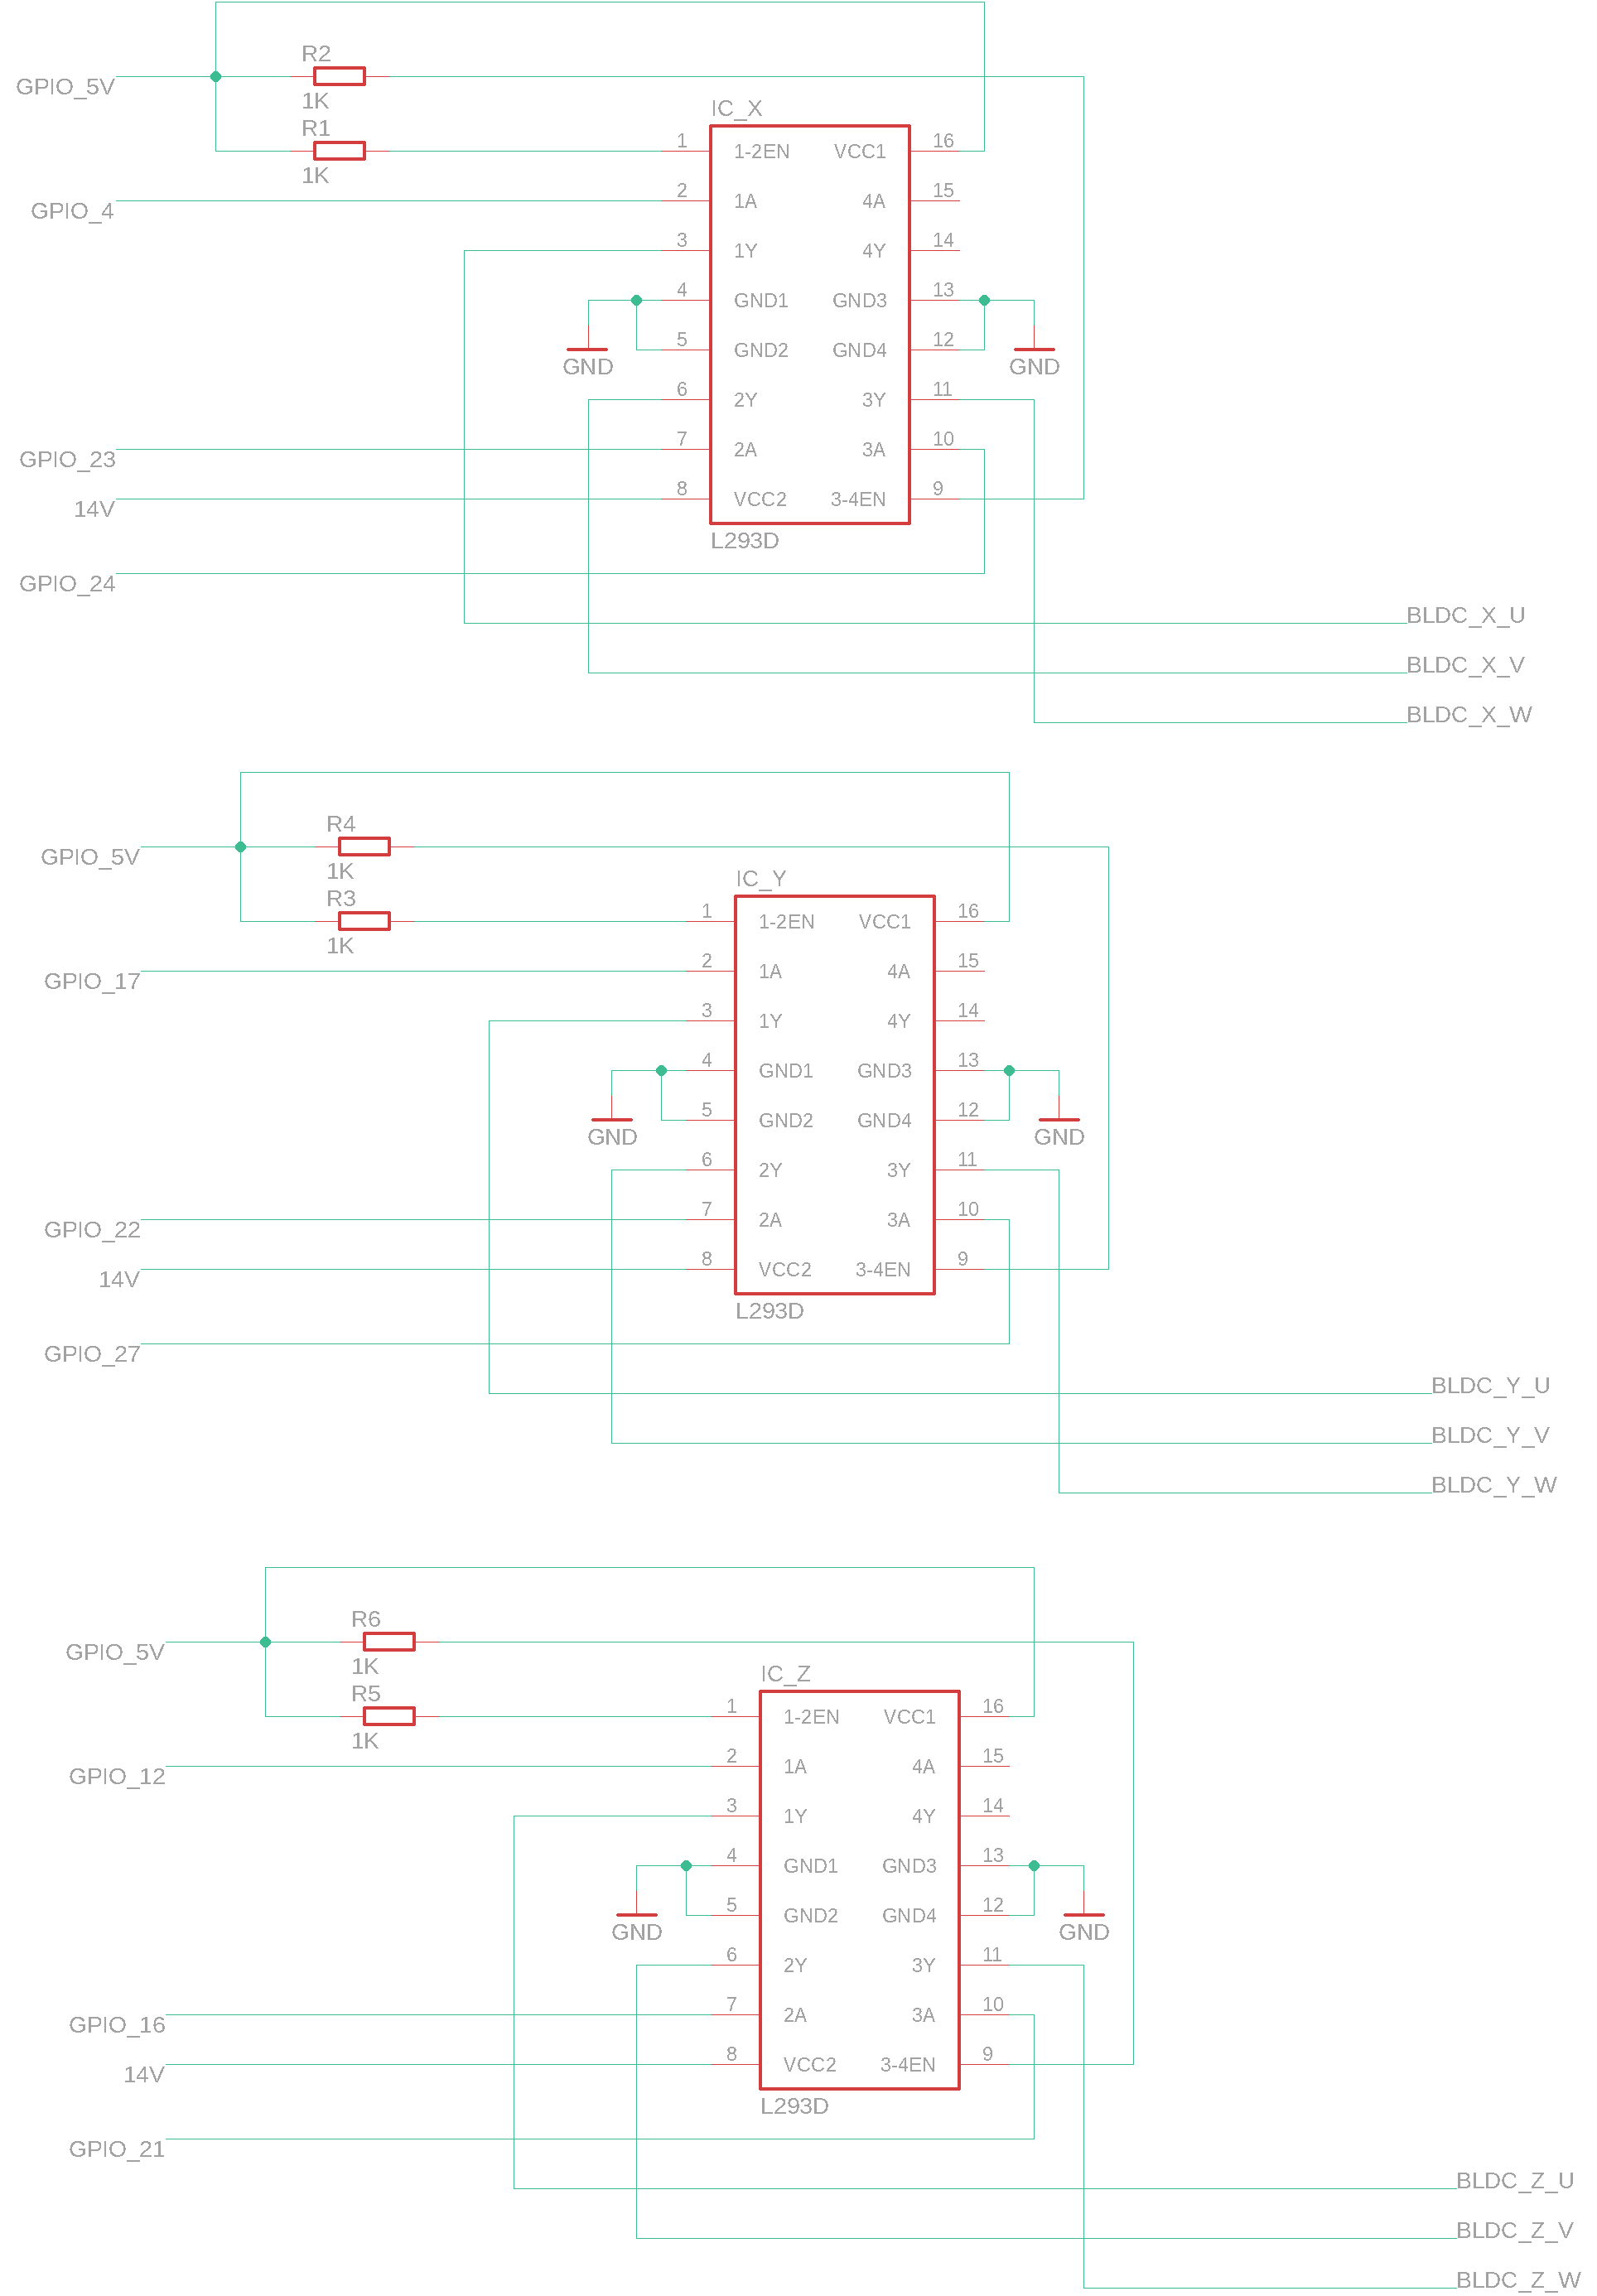
\includegraphics[width=0.7\linewidth]{ICschaltung.PNG}
	\caption[Schaltplan der Steuerung, erstellt von Erik Rother, 03.09.2018]{Schaltplan der Steuerung}
	\label{fig:mikrocontroller-schaltung}
\end{figure}
% Literatur
\renewcommand\refname{Literaturverzeichnis}
\addtocontents{toc}{\vspace{-0.5em}}

\bibliographystyle{alphadin}

\newpage
\bibliography{literatur}

%Abbildungen
\listoffigures

%Tabellen
\listoftables

\end{document}
